\documentclass[12pt]{article}
\pdfminorversion=7

\usepackage[letterpaper,top=0.8in,bottom=0.85in,left=1in,right=1in]{geometry}
\usepackage{amsmath,amssymb,amsthm,mathtools,aliascnt}
\usepackage[T1]{fontenc}
\usepackage{mathptmx}
\usepackage{microtype}
\usepackage{setspace}
\usepackage{booktabs,longtable,array,tabularx,multirow}
\usepackage{graphicx}
\usepackage{float}
\usepackage{caption}
\usepackage{subcaption}
\usepackage{enumitem}
\usepackage{pdflscape}
\usepackage{xurl}
\usepackage{listings}
\usepackage{xcolor}
\usepackage{tikz}
\usetikzlibrary{arrows.meta,positioning,calc,fit}
\usepackage{titlesec}
\usepackage[section]{placeins}
\usepackage[hidelinks]{hyperref}
\usepackage[nameinlink,capitalise]{cleveref}
\usepackage[authoryear,round]{natbib}
\let\parencite\citep
\let\textcite\citet

\hypersetup{
  pdftitle={Boundary Limited Observer Systems: Empirical Equivalence, Interface Refinement, and the Limits of Latent Reconstruction},
  pdfauthor={Christopher Ezernack},
  pdfsubject={Observer interfaces, empirical equivalence, latent nonidentifiability, and reconstruction limits}
}

\pagestyle{plain}
\urlstyle{same}
\setstretch{1.06}
\setlength{\parindent}{0.25in}
\setlength{\parskip}{0pt}
\setlength{\emergencystretch}{2em}
\widowpenalty=10000
\clubpenalty=10000
\displaywidowpenalty=10000
\setcounter{topnumber}{3}
\setcounter{bottomnumber}{2}
\setcounter{totalnumber}{5}
\renewcommand{\topfraction}{0.9}
\renewcommand{\bottomfraction}{0.8}
\renewcommand{\textfraction}{0.07}
\renewcommand{\floatpagefraction}{0.82}
\renewcommand{\arraystretch}{1.12}

\titleformat{\section}
  {\normalfont\large\bfseries}
  {\thesection.}{0.55em}{}
\titleformat{\subsection}
  {\normalfont\normalsize\bfseries}
  {\thesubsection}{0.55em}{}
\titleformat{\subsubsection}
  {\normalfont\normalsize\itshape}
  {\thesubsubsection}{0.55em}{}
\titlespacing*{\section}{0pt}{2.0ex plus .4ex minus .2ex}{0.8ex}
\titlespacing*{\subsection}{0pt}{1.6ex plus .3ex minus .2ex}{0.5ex}
\titlespacing*{\subsubsection}{0pt}{1.3ex plus .2ex minus .2ex}{0.4ex}

\captionsetup{
  font=small,
  labelfont=bf,
  labelsep=period,
  justification=raggedright,
  singlelinecheck=false,
  skip=6pt
}
\captionsetup[subfigure]{font=footnotesize,labelfont=bf,justification=centering}
\setlist{nosep,leftmargin=2em}

\theoremstyle{definition}
\newtheorem{definition}{Definition}[section]
\theoremstyle{plain}
\newaliascnt{proposition}{definition}
\newtheorem{proposition}[proposition]{Proposition}
\aliascntresetthe{proposition}
\crefname{proposition}{proposition}{propositions}
\Crefname{proposition}{Proposition}{Propositions}
\newaliascnt{theorem}{definition}
\newtheorem{theorem}[theorem]{Theorem}
\aliascntresetthe{theorem}
\crefname{theorem}{theorem}{theorems}
\Crefname{theorem}{Theorem}{Theorems}
\newaliascnt{corollary}{definition}
\newtheorem{corollary}[corollary]{Corollary}
\aliascntresetthe{corollary}
\crefname{corollary}{corollary}{corollaries}
\Crefname{corollary}{Corollary}{Corollaries}
\newaliascnt{lemma}{definition}
\newtheorem{lemma}[lemma]{Lemma}
\aliascntresetthe{lemma}
\crefname{lemma}{lemma}{lemmas}
\Crefname{lemma}{Lemma}{Lemmas}
\theoremstyle{remark}
\newaliascnt{remark}{definition}
\newtheorem{remark}[remark]{Remark}
\aliascntresetthe{remark}
\crefname{remark}{remark}{remarks}
\Crefname{remark}{Remark}{Remarks}
\theoremstyle{definition}
\newaliascnt{hypothesis}{definition}
\newtheorem{hypothesis}[hypothesis]{Hypothesis}
\aliascntresetthe{hypothesis}
\crefname{hypothesis}{hypothesis}{hypothesiss}
\Crefname{hypothesis}{Hypothesis}{Hypothesiss}
\newaliascnt{researchquestion}{definition}
\newtheorem{researchquestion}[researchquestion]{Research Question}
\aliascntresetthe{researchquestion}
\crefname{researchquestion}{research question}{research questions}
\Crefname{researchquestion}{Research Question}{Research Questions}

\newcommand{\Obs}{\mathcal O}
\newcommand{\Out}{\mathcal R}
\newcommand{\Emp}{\mathcal E}
\newcommand{\id}{\operatorname{id}}
\newcommand{\im}{\operatorname{im}}
\newcommand{\card}{\operatorname{card}}
\newcommand{\Reach}{\operatorname{Reach}}
\newcommand{\Model}{\mathsf M}
\newcommand{\Extended}{\mathsf M^{\ast}}
\newcommand{\bool}{\{0,1\}}


\newenvironment{proofstatement}
{\begin{quote}\small\noindent\textbf{Proof statement.}\ }
{\end{quote}}

\lstdefinelanguage{Python}{
  morekeywords={def,return,for,in,if,not,and,True,False,class,property},
  sensitive=true,
  morecomment=[l]{\#},
  morestring=[b]",
  morestring=[b]'
}
\lstdefinelanguage{Lean}{
  morekeywords={theorem,def,structure,abbrev,where,by,let,have,exact,refine,constructor,fun,forall,exists,Type,Prop,Nonempty},
  sensitive=true,
  morecomment=[l]{--},
  morecomment=[s]{/-}{-/},
  morestring=[b]"
}
\lstset{
  language=Python,
  basicstyle=\ttfamily\small,
  keywordstyle=\bfseries,
  commentstyle=\itshape,
  columns=fullflexible,
  keepspaces=true,
  frame=single,
  framerule=0.35pt,
  rulecolor=\color{black!45},
  backgroundcolor=\color{black!2},
  breaklines=true,
  showstringspaces=false,
  aboveskip=8pt,
  belowskip=8pt
}

\begin{document}

\begin{flushleft}
{\large Christopher Ezernack}\par
\small Department of Physics and Cognitive Science, The University of Texas at Dallas\par
\small \texttt{christopher.ezernack@utdallas.edu}\par
\vspace{1.25em}
{\LARGE\bfseries Boundary Limited Observer Systems\par}
\vspace{0.3em}
{\large Empirical Equivalence, Interface Refinement, and the Limits of Latent Reconstruction\par}
\vspace{0.55em}
\end{flushleft}
\vspace{0.5em}
\hrule
\vspace{0.8em}

\noindent\textbf{Abstract.}
An observation map can preserve every recorded output while failing to determine the latent state that produced it. We study this distinction for a deterministic interface \(\pi:X\to O\). Exact decoding requires a left inverse and therefore injectivity; quantities determined by the observation are constant on its fibers. At the model level, we define empirical equivalence as equality of reachable observation sets. For every model with a nonempty latent space, adjoining an unobserved Boolean coordinate gives an equivalent model without an exact decoder. If the original is exactly decodable, the two models have opposite decoder statuses. Interface refinement describes which additional distinctions a measurement can retain. Exhaustive finite calculations reproduce the hidden multiplicities, collision counts, and refinement maps, and agree with twelve archived output tables. The result concerns set based identifiability within the declared model class. It does not establish equality of probability laws, impossibility of reconstruction from temporal measurements, or physical existence of the added coordinate. The proofs and computational details are supplied in appendices and a companion supplement.

\medskip
\noindent\textbf{Keywords:} observer interface; reachable observations; latent reconstruction; identifiability; quotient; interface refinement.


\section{Introduction}
\label{sec:mainintro}
Scientific measurements represent selected features of a system. A measurement can be accurate for its intended purpose while leaving several source states compatible with the same output. The resulting inverse problem depends on the observation map, the allowed model class, and the quantity to be reconstructed.

Identifiability theory asks which model properties observations determine. Statistical formulations compare probability laws, while dynamical observability uses outputs together with specified evolution and inputs \parencite{Rothenberg1971,HermannKrener1977}. The present analysis isolates a simpler question: what follows from a deterministic observation map and the set of outputs it can produce? This restriction permits exact statements about fibers, reconstruction, and comparison of interfaces.

The main construction appends a coordinate that the observation map ignores. The extended model produces the same reachable observations, but distinct hidden labels prevent exact reconstruction. The construction proves nonuniqueness within a model class that permits such extensions. Additional dynamics, interventions, or physical constraints may exclude them. Related limits in learned latent representations likewise depend on the assumptions imposed on the model class \parencite{Locatello2019}.

The contribution is a unified formalization of these set theoretic facts, their refinement relations, and their finite computational witnesses. It does not establish a general impossibility of self-observation or a theory of consciousness. Section~\ref{sec:mainframework} defines the model and principal equations. Section~\ref{sec:mainresult} states the main result. Sections~\ref{sec:mainmethods} and~\ref{sec:mainfindings} give the methods and findings, followed by their implications and conclusion. Detailed proofs, counterexamples, and the broader research program follow in the appendices.

\section{Observation model and principal equations}
\label{sec:mainframework}
An interface is a map \(\pi:X\to O\) from a source state space to an observation space. Two states are observationally equivalent when their outputs agree:
\begin{equation}
x\sim_\pi y\ \Longleftrightarrow\ \pi(x)=\pi(y),
\qquad Q_\pi=X/{\sim_\pi}.
\label{eq:stateequivalence}
\end{equation}
Each class is a fiber of \(\pi\). The quotient \(Q_\pi\) is bijective with the reachable range \(\pi[X]\). A quantity \(f:X\to V\) is determined on that range precisely when it is constant on every fiber, equivalently when it factors uniquely through the quotient. This is a statement about set functions; it supplies no algorithm or error bound.

A globally exact decoder is a total map \(d:O\to X\) satisfying
\begin{equation}
d\circ\pi=\id_X\quad\Longrightarrow\quad\pi\text{ is injective}.
\label{eq:decoder}
\end{equation}
When \(X\neq\varnothing\), injectivity is also sufficient: invert \(\pi\) on its range and use one fixed state on unreachable observations. When \(X=\varnothing\), a total decoder exists exactly when \(O=\varnothing\). The definitions distinguish a decoder on all of \(O\) from one defined only on reachable observations.

A model \(\Model=(X_\Model,\pi_\Model)\) has reachable set \(\Obs(\Model)=\pi_\Model[X_\Model]\). Models with the same observation codomain are compared by
\begin{equation}
\Model\approx\Model'\ \Longleftrightarrow\
\Obs(\Model)=\Obs(\Model').
\label{eq:modelequivalence}
\end{equation}
Throughout this paper, \emph{empirical equivalence} means this equality of reachable sets. No probability law is part of the definition. An admissible experiment is a fixed function \(e:O\to R\) that processes an observation. Its possible outcomes are
\begin{equation}
\Out_e(\Model)=e[\Obs(\Model)],\qquad
\Model\approx\Model'\ \Longrightarrow\
\Out_e(\Model)=\Out_e(\Model').
\label{eq:outcomes}
\end{equation}
Such an experiment neither changes the source dynamics nor acquires another measurement. Interventions and temporal records require an enlarged model.

Interfaces on the same source space can retain different distinctions. A fine interface \(\pi_F:X\to O_F\) refines \(\pi_C:X\to O_C\) when a coarsening map \(c\) satisfies
\begin{equation}
\pi_C=c\circ\pi_F.
\label{eq:refinement}
\end{equation}
This relation is reflexive and transitive. It induces a surjection \([x]_F\mapsto[x]_C\) between observable quotients. If a pair is separated by \(F\) and merged by \(C\), that quotient map is noninjective and reverse refinement is impossible. The proofs are in \Cref{sec:interfaces,sec:observablequotient,sec:refinement}.

\section{Main result: equivalent outputs and nonunique latent models}
\label{sec:mainresult}
The hidden extension makes the reconstruction limit explicit. For a model with \(X_\Model\neq\varnothing\), define
\begin{equation}
X_{\Extended}=X_\Model\times\{0,1\},\qquad
\pi_{\Extended}(x,b)=\pi_\Model(x),\qquad p(x,b)=x.
\label{eq:extension}
\end{equation}
The map \(p\) is surjective and preserves observations. Distinct Boolean labels over the same base state produce a collision.

\begin{theorem}[Hidden extension and reconstruction]
For every model with a nonempty latent space, the extension in \eqref{eq:extension} has the same reachable set and the same possible outcomes under every fixed observation processing map \(e\). It has no globally exact decoder. If the base has an exact decoder, the two models have different decoder statuses.
\label{thm:mainhidden}
\end{theorem}

The proof follows from two identities. Each base output is produced by \((x,0)\), and every extended output is a base output. Meanwhile, \((x,0)\) and \((x,1)\) are distinct states with the same observation. Equation~\eqref{eq:decoder} excludes a decoder. The complete construction and supporting results appear in \Cref{sec:hidden,sec:synthesis}.

For \(O\neq\varnothing\), compare the identity model \((O,\id_O)\) with its Boolean extension. Both reach all of \(O\), but only the identity model has an exact decoder. Thus no function of the reachable set can determine decoder existence for every model in a class containing both. This does not mean that every equivalence class contains both statuses, nor that adjoining a hidden coordinate changes the status of an already nondecodable base.

The same limitation holds for a complete family of Boolean predicates on observations. A predicate records whether it succeeds at any reachable output. Agreement for all predicates is equivalent to reachable-set equality, because predicates testing equality to individual observations determine membership. Model properties descend to the empirical quotient exactly when they are constant on its classes. These statements are proved in \Cref{sec:predicates,sec:empiricalquotient}.

\section{Methods}
\label{sec:mainmethods}
The study combines deductive proofs with exhaustive finite calculations. The calculations enumerate declared mathematical models; no biological measurements or physical parameter estimates enter the analysis. The reference code is \texttt{BoundaryObserver} at commit \nolinkurl{eb96b984ae999ee6cbc0aae33c2d501c46d9540f}. The formal source remains unchanged in this revision.

The finite base has \(X=O=\{0,1,2,3,4,5\}\) and \(\pi(x)=x\). A comparison model observes \(x\bmod3\). Hidden extensions use \(m\in\{1,2,3,5,8\}\) labels for each base state, with \(\pi_m(x,h)=x\). For each reachable output, the program enumerates its fiber and calculates
\begin{equation}
C(\Model)=\sum_{o\in\Obs(\Model)}\binom{|\pi_\Model^{-1}(o)|}{2},
\qquad C(\Model_m)=3m(m-1).
\label{eq:collisions}
\end{equation}
The collision count measures unordered pairs with equal outputs. It is not a probability or an entropy.

Four processing maps test identity, a threshold at three, a three category partition, and width two compression. Three predicates test evenness, values at least three, and membership in \(\{0,5\}\). A separate eight state example compares identity, paired buckets, binary regions, and a relabeled identity. Every claimed finite relation is evaluated over its full declared domain.

The revision reruns the eighteen repository tests and six additional tests of the assumptions and counterexamples. It also regenerates all twelve CSV outputs and compares their bytes with the archived files. The repository records successful Lean CI for the pinned commit; a new Lean build is not claimed here. The added examples have explicit proofs in \Cref{app:scopechecks} and are not represented as newly checked Lean declarations. Commands, exact outputs, and declaration correspondence are supplied in the package and companion supplement.

\section{Findings}
\label{sec:mainfindings}
The finite calculations reproduce the predicted separation between latent multiplicity and reachable outputs. The injective base has six singleton fibers and a decoder. Its Boolean extension has twelve states, six two-state fibers, and no decoder. The modulo three comparison has three reachable outputs, three collisions, and no decoder.

\begin{table}[htbp]
\centering\small
\caption{Exhaustive hidden extension calculations. Each row reaches the same six observations.}
\label{tab:mainmultiplicity}
\begin{tabular}{@{}rrrrrl@{}}
\toprule
\(m\)&Latent states&Reachable outputs&Fiber size&Collisions&Exact decoder\\
\midrule
1&6&6&1&0&Yes\\
2&12&6&2&6&No\\
3&18&6&3&18&No\\
5&30&6&5&60&No\\
8&48&6&8&168&No\\
\bottomrule
\end{tabular}
\end{table}

All twenty eight model and experiment comparisons preserve the corresponding outcome set. All twenty one existential predicate comparisons and all twenty one complete truth-table comparisons agree with the base. These three selected predicates illustrate invariance; the theorem concerning every predicate is established separately by proof.

Refinement retains eight, four, and two observable classes for identity, paired buckets, and binary regions. Identity to paired, paired to region, and identity to region respectively collapse four, eight, and twelve previously distinguished pairs. Each induced quotient map is surjective and noninjective. Relabeling preserves all eight classes and gives a bijection. Complete tables and figures appear in \Cref{sec:results} and the supplement.

All twenty four tests pass. The twelve regenerated CSV files are byte identical to the archived outputs. The finite counts use exact enumeration and integer arithmetic. They have no integration step, sampling uncertainty, or asymptotic numerical convergence claim. Exhaustive agreement for these examples does not establish a result for every model; the general conclusions depend on the proofs.

\section{Discussion}
\label{sec:maindiscussion}
The result identifies a restriction on inference from a specified interface. If a quantity varies within an observation fiber, that observation alone cannot determine it exactly. A stronger reconstruction claim must state the assumptions that eliminate the ambiguity. Such assumptions may include known dynamics, additional sensors, interventions, regularity, or a justified restriction of the latent model class.

Equality of reachable sets is weaker than statistical equivalence. Bernoulli laws with parameters \(1/10\) and \(9/10\) both permit the outputs zero and one, but assign different probabilities to them. The present definition omits that distinction. A statistical extension must compare induced probability laws or likelihoods rather than only possible outputs \parencite{Rothenberg1971}.

An instantaneous collision also need not prevent reconstruction from time dependent observations. For the known system
\begin{equation}
\dot x_1=x_2,\qquad\dot x_2=0,\qquad y=x_1,
\end{equation}
one output leaves \(x_2\) undetermined, while \(y(0)\) and \(y(T)\), for \(T\neq0\), determine both initial coordinates. Measurement error in the reconstructed second coordinate is amplified as \(|T|\) becomes small. The derivation and error bound are in \Cref{app:scopechecks}. This distinction is consistent with dynamical observability theory \parencite{HermannKrener1977}.

Neural applications require the same separation between source state, measurement, and reconstruction. Published grid-cell studies motivate analysis of how population geometry depends on the measurement interface \parencite{Gardner2022}. A spatial tuning map, a temporal population trajectory, a topological reconstruction, and evidence of attraction are different objects. The present set theoretic result supplies no inference from toroidal geometry to an attracting invariant torus. That inference requires specified dynamics and evidence concerning invariance and stability.

The hidden coordinate is a mathematical witness permitted by the model class. Its construction does not demonstrate an unmeasured physical variable. Questions about embedded self-modeling, consciousness, or continuity across scales require additional definitions and observations. They are retained as a research program in \Cref{sec:limitations,app:motivation}, with their status separated from the theorem.

\section{Conclusion}
\label{sec:mainconclusion}
A declared observation map determines a partition of source states. Exact reconstruction requires that the map preserve every source distinction, and reachable-set equality does not determine decoder existence across an unrestricted class of latent models. The Boolean extension supplies a constructive witness, while interface refinement describes how a richer measurement can preserve distinctions lost by a coarser one.

The finite calculations reproduce the stated counts and invariance relations. The scope of the result remains deterministic and set based. Probability laws, temporal measurements, physical constraints, and reconstruction error must be specified before applying it to a scientific system. The resulting practical question is which additional measurement or model assumption would separate the states relevant to the proposed inference.


\clearpage
\appendix
\section{Mathematical preliminaries and proof convention}
\label{sec:preliminaries}

\subsection{Functions, images, and fibers}

The notation for functions, images, fibers, composition, inverses, and equivalence relations follows standard set-theoretic usage \parencite[Chs. 8--11]{Halmos1974}. For a function \(f:X\to Y\), the image of a subset \(A\subseteq X\) is
\[
f[A]=\{f(x):x\in A\}.
\]
The range is \(\im(f)=f[X]\). The fiber over \(y\in Y\) is
\[
f^{-1}(y)=\{x\in X:f(x)=y\}.
\]
The function is injective when \(f(x)=f(x')\) implies \(x=x'\). It is surjective when every \(y\in Y\) has at least one preimage.

A function \(g:Y\to X\) is a left inverse of \(f\) when
\[
g\circ f=\id_X.
\]
A left inverse can exist only when \(f\) is injective \parencite[Chs. 1 and 4]{MacLaneBirkhoff1999}. This elementary fact is the exact-decoding obstruction used throughout the paper.

\subsection{Equivalence relations and quotients}

An equivalence relation partitions a set into disjoint equivalence classes. The quotient \(X/{\sim}\) is the set of those classes. The canonical class map is
\[
q:X\to X/{\sim},
\qquad
q(x)=[x].
\]
A function on \(X\) descends to the quotient precisely when it is constant on each equivalence class. The descended function is then unique because every quotient class has a representative. This is the elementary set-level form of a quotient universal property \parencite{MacLaneBirkhoff1999,Leinster2014}.

\subsection{State-level and model-level notation}

The symbol \(X\) denotes a source or world state space. The symbol \(O\) denotes an accessible observation space. The observation map is \(\pi:X\to O\). A generative model is written
\[
\Model=(X_\Model,\pi_\Model).
\]
Its reachable observation set is \(\Obs(\Model)\). The possible outcome set of an admissible experiment \(e\) is \(\Out_e(\Model)\).

Two equivalence relations are used. State-level observational equivalence identifies \(x,y\in X\) when \(\pi(x)=\pi(y)\). Model-level empirical equivalence identifies \(\Model\) and \(\Model'\) when \(\Obs(\Model)=\Obs(\Model')\). The levels are not interchangeable.

\subsection{Logical status of statements}

Definitions fix the objects and relations used in the analysis. Propositions, lemmas, corollaries, and theorems are established by the proofs that follow them. Finite computations evaluate explicitly enumerated instances of those definitions. Interpretations, hypotheses, applications, and future research questions are stated separately and do not inherit proof from the mathematical results. Literature citations identify established precedent, comparison, or empirical context.

\section{Observer interfaces, accessible quantities, and exact decoding}
\label{sec:interfaces}

A single observation map determines which states produce the same output. In dynamical observability, the available evidence is an output trajectory generated by specified dynamics and inputs \parencite{Kalman1963,HermannKrener1977,Sontag1998}.

\begin{definition}[Observer interface]
An observer interface on a world state space \(X\) is a pair
\[
I=(O,\pi),
\]
where \(O\) is an accessible observation space and \(\pi:X\to O\) is the observation map.
\end{definition}
\begin{definition}[Observational equivalence]
For \(x,y\in X\), define
\[
x\sim_I y
\quad\Longleftrightarrow\quad
\pi(x)=\pi(y).
\]
\end{definition}
\begin{proposition}
Observational equivalence is reflexive, symmetric, and transitive.
\end{proposition}

\begin{proof}
Reflexivity follows from \(\pi(x)=\pi(x)\). Symmetry follows because equality is symmetric. Transitivity follows because \(\pi(x)=\pi(y)\) and \(\pi(y)=\pi(z)\) imply \(\pi(x)=\pi(z)\).
\end{proof}
The equivalence class of \(x\) is the fiber
\[
[x]_I=\pi^{-1}(\pi(x)).
\]
The class contains exactly the source states that the interface represents by the same accessible value. Equivalence is therefore relative to \(I\). A second interface may separate states that the first interface merges.

\subsection{Quantities that factor through the interface}

An accessible quantity is a set function of the observation. Computability, cost, and stability under measurement error require additional hypotheses.

\begin{definition}[Interface accessible quantity]
Let \(q:X\to V\). The quantity \(q\) factors through \(I\) when there exists a map \(\bar q:O\to V\) such that
\[
q=\bar q\circ\pi.
\]
\end{definition}
\begin{theorem}[Fiber constancy]
If \(q\) factors through \(I\), then \(q\) is constant on every observation fiber. In particular,
\[
x\sim_I y
\quad\Longrightarrow\quad
q(x)=q(y).
\]
\end{theorem}

\begin{proof}
Assume \(q=\bar q\circ\pi\). Let \(x\sim_I y\). By definition, \(\pi(x)=\pi(y)\). Applying \(\bar q\) to both sides gives
\[
\bar q(\pi(x))=\bar q(\pi(y)).
\]
Substitution of \(q=\bar q\circ\pi\) yields \(q(x)=q(y)\).
\end{proof}
A quantity constant on every fiber has a unique representation on the observable quotient (\Cref{sec:observablequotient}).

\begin{corollary}[Variation prevents interface factorization]
If \(x\sim_I y\) and \(q(x)\neq q(y)\), then \(q\) does not factor through \(I\).
\end{corollary}

\begin{proof}
If \(q\) factored through \(I\), fiber constancy would imply \(q(x)=q(y)\), contradicting the assumption.
\end{proof}
\subsection{Internal tests}

An internal test is a special case of an accessible quantity.

\begin{definition}[Internal test]
An internal binary test is a function
\[
t:O\to\{\mathrm{false},\mathrm{true}\}.
\]
\end{definition}
\begin{proposition}[No internal test separates one fiber]
If \(x\sim_I y\), then
\[
t(\pi(x))=t(\pi(y))
\]
for every internal test \(t\).
\end{proposition}

\begin{proof}
Apply \(t\) to both sides of \(\pi(x)=\pi(y)\).
\end{proof}
Every test on \(O\) receives the same input for states in one fiber. Changing its output space cannot distinguish these states.

\subsection{Exact reconstruction}

An exact decoder is a left inverse of the observation map \parencite[Chs. 10--11]{Halmos1974}.

\begin{definition}[Globally exact decoder]
A globally exact decoder for \(I\) is a function \(d:O\to X\) such that
\[
d\circ\pi=\id_X.
\]
\end{definition}
\begin{theorem}[Exact decoding implies injectivity]
If a globally exact decoder exists, then \(\pi\) is injective.
\label{thm:decoderinjective}
\end{theorem}

\begin{proof}
Assume \(d\circ\pi=\id_X\). Let \(x,y\in X\) and assume \(\pi(x)=\pi(y)\). Applying \(d\) gives
\[
d(\pi(x))=d(\pi(y)).
\]
The left inverse condition reduces this equality to \(x=y\). Therefore \(\pi\) is injective.
\end{proof}
\begin{corollary}[Noninjectivity prevents exact decoding]
If \(\pi\) is noninjective, then no globally exact decoder exists.
\end{corollary}

\begin{proof}
The statement is the contrapositive of \Cref{thm:decoderinjective}.
\end{proof}
A many to one observation may still identify a particular target or identify a state within a restricted source class.

\subsection{Finite capacity obstruction}

For finite sets, counting the possible outputs can rule out injectivity.

\begin{theorem}[Finite pigeonhole obstruction]
Let \(X\) and \(O\) be finite. If
\[
|O|<|X|,
\]
then every observation map \(\pi:X\to O\) is noninjective. Therefore there exist distinct \(x,y\in X\) such that \(x\sim_I y\), and no globally exact decoder exists.
\end{theorem}

\begin{proof}
Assume for contradiction that \(\pi\) is injective. An injective map from a finite set \(X\) into a finite set \(O\) implies \(|X|\leq |O|\). This contradicts \(|O|<|X|\). Hence \(\pi\) is noninjective. The collision and decoder conclusions follow from the definitions and the preceding corollary.
\end{proof}


\section{The observable quotient and universal factorization}
\label{sec:observablequotient}

The observation map induces a canonical representation of the distinctions retained by the interface. The representation is the quotient of \(X\) by observational equivalence. Quotient sets and their representative-independent maps are standard constructions \parencite[Chs. 8--11]{Halmos1974}; the factorization language used below follows the universal-property viewpoint \parencite{MacLaneBirkhoff1999,Leinster2014}.

\begin{definition}[Observable quotient]
The observable quotient of \(X\) relative to \(I\) is
\[
Q_I=X/{\sim_I}.
\]
The canonical class map is
\[
q_I:X\to Q_I,
\qquad
q_I(x)=[x]_I.
\]
\end{definition}
The quotient discards the identities of states inside each fiber and retains the partition induced by observation. It is neither larger nor smaller than the available distinctions in the following sense.

\begin{proposition}[Quotient equality]
For \(x,y\in X\),
\[
q_I(x)=q_I(y)
\quad\Longleftrightarrow\quad
x\sim_I y.
\]
\end{proposition}

\begin{proof}
Two quotient classes are equal exactly when their representatives are related by the defining equivalence relation. Here that relation is equality of observations.
\end{proof}
Let \(\im(\pi)\subseteq O\) denote the reachable observation range. Each quotient class has one observation value, and each reachable observation value has one quotient class.

\begin{theorem}[Canonical equivalence with the observation range]
The map
\[
\Phi:Q_I\to\im(\pi),
\qquad
\Phi([x]_I)=\pi(x),
\]
is well defined and bijective.
\end{theorem}

\begin{proof}
Well definedness follows because representatives of one class have equal observations. Surjectivity follows from the definition of \(\im(\pi)\). For injectivity, suppose \(\Phi([x]_I)=\Phi([y]_I)\). Then \(\pi(x)=\pi(y)\), so \(x\sim_I y\) and \([x]_I=[y]_I\).
\end{proof}
The quotient and the reachable range are therefore equivalent descriptions of accessible resolution. The quotient emphasizes which source states have been identified. The range emphasizes which observation values remain reachable.

\begin{figure}[tbp]
\centering
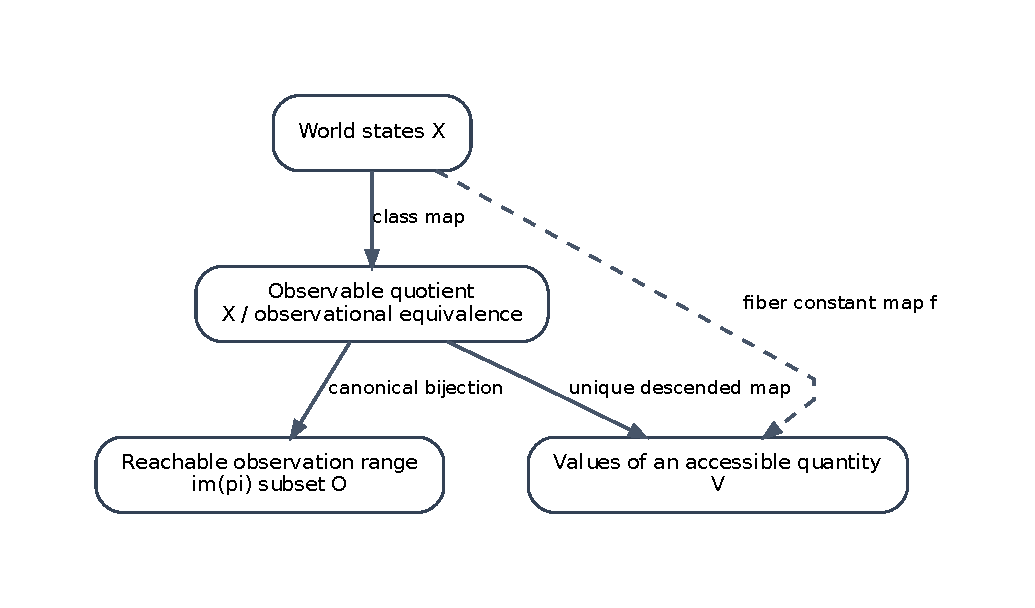
\includegraphics[width=0.88\textwidth]{figures/concept_observable_quotient.pdf}
\caption{Universal factorization through the observable quotient. A quantity defined on world states descends uniquely to the quotient exactly when it is constant on observation fibers. The quotient is canonically equivalent to the reachable observation range.}
\label{fig:observablequotient}
\end{figure}

\subsection{Universal property}

The quotient is characterized by a universal property. Universal properties identify an object by the unique maps that factor through it rather than by a choice of representatives \parencite{Leinster2014}.

\begin{theorem}[Observable quotient universal property]
Let \(f:X\to V\). The following statements are equivalent.
\begin{enumerate}[label=(\roman*)]
\item \(f(x)=f(y)\) whenever \(x\sim_I y\).
\item There exists a unique map \(\bar f:Q_I\to V\) such that
\[
f=\bar f\circ q_I.
\]
\end{enumerate}
\label{thm:observableuniversal}
\end{theorem}

\begin{proof}
Assume (i). Define \(\bar f([x]_I)=f(x)\). The definition is independent of the representative because \(f\) is constant on each equivalence class. For every \(x\in X\),
\[
(\bar f\circ q_I)(x)=\bar f([x]_I)=f(x),
\]
so the factorization exists. If \(g:Q_I\to V\) also satisfies \(f=g\circ q_I\), then for every class \([x]_I\),
\[
g([x]_I)=g(q_I(x))=f(x)=\bar f([x]_I).
\]
Thus \(g=\bar f\), proving uniqueness.

Conversely, assume (ii) and let \(x\sim_I y\). Then \(q_I(x)=q_I(y)\). Therefore
\[
f(x)=\bar f(q_I(x))=\bar f(q_I(y))=f(y).
\]
Hence \(f\) is constant on each fiber.
\end{proof}
The theorem provides a precise meaning for ``observer accessible.'' A quantity is determined on reachable observations exactly when it is a function of the observable equivalence class. Any quantity that varies inside a class requires information not present in that quotient.

\subsection{Composition with the observation range}

The original definition of interface factorization used a map \(\hat f:O\to V\). The quotient theorem uses a map \(\bar f:Q_I\to V\). These formulations agree on reachable observations. Extension to all of \(O\) is automatic when \(V\neq\varnothing\), by choosing a value on unreachable observations. If \(V=\varnothing\), a map \(X\to V\) requires \(X=\varnothing\); a map \(O\to V\) then exists only if \(O=\varnothing\). A function on the full codomain \(O\) may assign arbitrary values to unreachable observations, while a function on \(Q_I\) contains only empirically realized classes. The distinction becomes useful at the model level, where the empirical quotient is represented exactly by realizable reachable sets.

\section{Interface refinement and information ordering}
\label{sec:refinement}

Different instruments or representational procedures may observe the same world at different resolutions. Interface refinement is a preorder on interfaces. Identifying mutually refining interfaces gives an order on the corresponding classes. This resembles comparison of statistical experiments by informativeness, but the present relation is deterministic and is defined by an explicit commuting coarsening map rather than by a Markov kernel or decision-risk criterion \parencite{Blackwell1951,Blackwell1953,Torgersen1991}.

Let
\[
F=(O_F,\pi_F)
\qquad\text{and}\qquad
C=(O_C,\pi_C)
\]
be interfaces on the same world state space \(X\).

\begin{definition}[Interface refinement]
The interface \(F\) refines \(C\), written
\[
F\succeq C,
\]
when there exists a coarsening map \(c:O_F\to O_C\) such that
\[
\pi_C=c\circ\pi_F.
\]
\end{definition}
The commuting equation states that every coarse observation is determined by a set function of the fine observation. It does not state that the fine observation can be recovered from the coarse observation.

\begin{proposition}[Refinement is reflexive and transitive]
Every interface refines itself. If \(F\succeq M\) and \(M\succeq C\), then \(F\succeq C\).
\end{proposition}

\begin{proof}
Reflexivity uses the identity map on \(O_F\). For transitivity, let \(a:O_F\to O_M\) and \(b:O_M\to O_C\) witness the two refinements. Then
\[
\pi_C=b\circ\pi_M=b\circ a\circ\pi_F,
\]
so \(b\circ a\) witnesses \(F\succeq C\).
\end{proof}
\subsection{Monotonicity of accessible structure}

Refinement orders observational equivalence in the expected direction.

\begin{theorem}[Fine equivalence implies coarse equivalence]
If \(F\succeq C\) and \(x\sim_F y\), then \(x\sim_C y\).
\end{theorem}

\begin{proof}
Let \(c\) witness the refinement. The equality \(\pi_F(x)=\pi_F(y)\) implies
\[
c(\pi_F(x))=c(\pi_F(y)).
\]
Using \(\pi_C=c\circ\pi_F\), this becomes \(\pi_C(x)=\pi_C(y)\).
\end{proof}
The converse need not hold. A coarse interface may identify states that a fine interface distinguishes.

\begin{theorem}[Factorization is monotone under refinement]
If \(F\succeq C\) and \(q:X\to V\) factors through \(C\), then \(q\) factors through \(F\).
\end{theorem}

\begin{proof}
Let \(q=\bar q_C\circ\pi_C\) and \(\pi_C=c\circ\pi_F\). Then
\[
q
=\bar q_C\circ c\circ\pi_F.
\]
Thus \(q\) factors through \(F\) by the map \(\bar q_F=\bar q_C\circ c\).
\end{proof}
Every coarse test can therefore be simulated from the fine observation. Exact reconstruction also moves in the same direction.

\begin{proposition}[A coarse decoder induces a fine decoder]
If \(F\succeq C\) and \(C\) has a globally exact decoder, then \(F\) has a globally exact decoder.
\end{proposition}

\begin{proof}
Let \(d_C:O_C\to X\) satisfy \(d_C\circ\pi_C=\id_X\), and let \(c:O_F\to O_C\) witness refinement. Define \(d_F=d_C\circ c\). Then
\[
d_F\circ\pi_F
=d_C\circ c\circ\pi_F
=d_C\circ\pi_C
=\id_X.
\]
\end{proof}
The contrapositive is useful: if the fine interface is noninjective, then no coarsening can be injective. Coarsening cannot restore a distinction that has already disappeared.

\subsection{Refinement maps between observable quotients}

Refinement induces a map between observable quotients.

\begin{figure}[tbp]
\centering
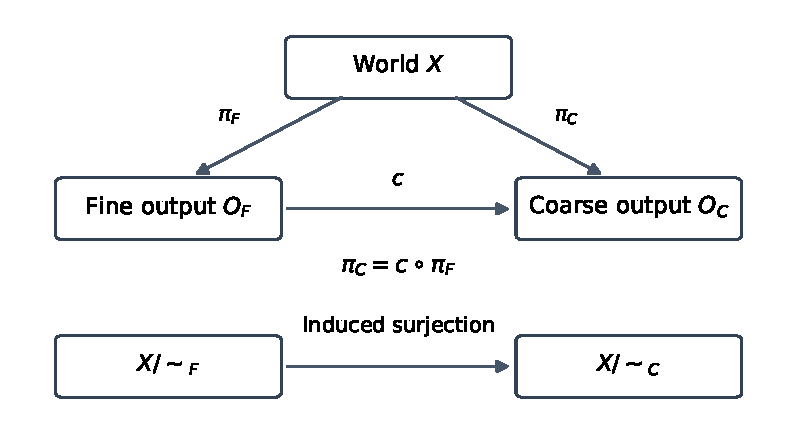
\includegraphics[width=0.88\textwidth]{figures/concept_interface_refinement.pdf}
\caption{Interface refinement and induced quotient map. The coarsening map makes the observation triangle commute. The induced map sends each fine observational class to its coarse class. The map is always surjective. Under strict refinement it is not injective.}
\label{fig:refinementdiagram}
\end{figure}

\begin{definition}[Induced quotient map]
If \(F\succeq C\), define
\[
Q_{F\to C}:X/{\sim_F}\longrightarrow X/{\sim_C}
\]
by
\[
Q_{F\to C}([x]_F)=[x]_C.
\]
\end{definition}
The map is well defined because fine equivalence implies coarse equivalence.

\begin{theorem}[Surjectivity of the quotient map]
For every refinement \(F\succeq C\), the map \(Q_{F\to C}\) is surjective.
\end{theorem}

\begin{proof}
Let \([x]_C\) be any coarse class. The fine class \([x]_F\) maps to it by definition:
\[
Q_{F\to C}([x]_F)=[x]_C.
\]
Therefore every coarse class has a fine preimage.
\end{proof}
\begin{definition}[Strict refinement]
The refinement \(F\succeq C\) is strict when there exist \(x,y\in X\) such that
\[
\pi_F(x)\neq\pi_F(y)
\qquad\text{and}\qquad
\pi_C(x)=\pi_C(y).
\]
\end{definition}
A strict refinement preserves at least one distinction that the coarse interface removes.

\begin{theorem}[Strict refinement makes the quotient map noninjective]
If \(F\) strictly refines \(C\), then \(Q_{F\to C}\) is not injective.
\end{theorem}

\begin{proof}
Choose \(x,y\) witnessing strictness. Since \(\pi_F(x)\neq\pi_F(y)\), the fine classes are distinct:
\[
[x]_F\neq[y]_F.
\]
Since \(\pi_C(x)=\pi_C(y)\), the coarse classes are equal. Hence
\[
Q_{F\to C}([x]_F)=[x]_C=[y]_C=Q_{F\to C}([y]_F),
\]
so the quotient map is noninjective.
\end{proof}
\begin{theorem}[Strict refinement prevents reverse refinement]
If \(F\) strictly refines \(C\), then \(C\) does not refine \(F\).
\end{theorem}

\begin{proof}
Suppose that \(C\succeq F\). Fine equivalence would then follow from coarse equivalence. The strictness witnesses satisfy \(x\sim_C y\) but \(x\not\sim_F y\), which is a contradiction.
\end{proof}
\subsection{Equal observational resolution}

Two interfaces can use different observation labels while preserving exactly the same partition of \(X\).

\begin{definition}[Same observational resolution]
Interfaces \(I\) and \(J\) have the same observational resolution when
\[
x\sim_I y
\quad\Longleftrightarrow\quad
x\sim_J y
\]
for every \(x,y\in X\).
\end{definition}
Mutual refinement implies equal observational resolution. Conversely, on reachable observations, equal resolution supplies mutually compatible class maps. The induced quotient maps are bijections.

\begin{theorem}[Mutual refinement gives quotient equivalence]
If \(I\succeq J\) and \(J\succeq I\), then the induced quotient maps are inverse bijections. Thus the two interfaces retain the same observational distinctions even when their observation representations differ.
\end{theorem}
This distinction separates strict coarsening from relabeling. Strict coarsening changes the partition of the world. Relabeling changes the symbols used for the classes but preserves the classes themselves.

\section{Generative models and admissible experiments}
\label{sec:models}

The state level framework extends to models with different latent spaces. The common comparison object is the accessible observation space. Comparing models by the outputs they can generate is adjacent to structural identifiability and statistical experiment theory, although the present definition uses equality of reachable sets rather than equality of distributions or parameterized trajectories \parencite{Rothenberg1971,WalterPronzato1997,Blackwell1951,Torgersen1991}.

\begin{definition}[Generative model]
A generative model over an observation space \(O\) is a pair
\[
\Model=(X_\Model,\pi_\Model),
\]
where \(X_\Model\) is the latent state space and \(\pi_\Model:X_\Model\to O\) is the observation map.
\end{definition}
\begin{definition}[Reachable observation set]
The reachable observation set of \(\Model\) is
\[
\Obs(\Model)
=
\{\pi_\Model(x):x\in X_\Model\}
=
\im(\pi_\Model).
\]
\end{definition}
\begin{definition}[Empirical equivalence]
Two models \(\Model\) and \(\Model'\) are empirically equivalent when
\[
\Model\approx\Model'
\quad\Longleftrightarrow\quad
\Obs(\Model)=\Obs(\Model').
\]
\end{definition}
Empirical equivalence is reflexive, symmetric, and transitive because set equality has those properties. The relation compares what the models can produce at the specified observation boundary. It does not compare latent identity directly.

\subsection{Observation only experiments}

An admissible experiment is intentionally restricted to the accessible observation. This follows the general methodological separation between an unobserved model state and the experiment or decision rule applied to its observable output \parencite{Blackwell1953,LeCam1986,LeCamYang2000}.

\begin{definition}[Admissible experiment]
An admissible experiment is a function
\[
e:O\to R.
\]
Its input is an accessible observation. It does not receive a latent state.
\end{definition}
\begin{definition}[Possible outcome set]
The possible outcome set of \(e\) under \(\Model\) is
\[
\Out_e(\Model)
=
\{e(\pi_\Model(x)):x\in X_\Model\}
=
e[\Obs(\Model)].
\]
\end{definition}
\begin{theorem}[Empirical equivalence preserves all admissible outcomes]
If \(\Model\approx\Model'\), then
\[
\Out_e(\Model)=\Out_e(\Model')
\]
for every admissible experiment \(e:O\to R\).
\label{thm:outcomeinvariance}
\end{theorem}

\begin{proof}
Empirical equivalence gives \(\Obs(\Model)=\Obs(\Model')\). Applying the same function \(e\) to equal sets gives
\[
e[\Obs(\Model)]=e[\Obs(\Model')].
\]
These images are the two possible outcome sets.
\end{proof}
The theorem applies to arbitrary result types. A Boolean test, categorical classifier, numerical compression, and identity map are all admissible experiments when their domain is \(O\).

\begin{definition}[Experimental separation]
An experiment separates \(\Model\) and \(\Model'\) when
\[
\Out_e(\Model)\neq\Out_e(\Model').
\]
\end{definition}
\begin{corollary}[No admissible separation inside one empirical class]
If \(\Model\approx\Model'\), no admissible experiment separates the models.
\end{corollary}
\subsection{The identity experiment}

The identity experiment retains the complete accessible observation value.

\begin{definition}[Identity experiment]
Define
\[
e_{\id}:O\to O,
\qquad
e_{\id}(o)=o.
\]
\end{definition}
\begin{proposition}
For every model \(\Model\),
\[
\Out_{e_{\id}}(\Model)=\Obs(\Model).
\]
\end{proposition}

\begin{proof}
The image of \(\Obs(\Model)\) under the identity function is \(\Obs(\Model)\) itself.
\end{proof}
The identity experiment is useful because it rules out an explanation based only on downstream compression. Even when the experiment returns every reachable accessible observation unchanged, the observation set may still fail to determine latent cardinality, fiber structure, or exact reconstructability.

\subsection{Properties determined by experiments}

Let \(P\) be a property of generative models. The property is determined by a fixed experiment \(e\) when there exists a criterion \(C\) on possible outcome sets such that
\[
P(\Model)
\quad\Longleftrightarrow\quad
C(\Out_e(\Model))
\]
for every model \(\Model\). Any property determined in this way is invariant under empirical equivalence, because empirically equivalent models have equal outcome sets.

This observation becomes decisive after strict hidden extensions are introduced. For \(O\neq\varnothing\), the identity model and its Boolean extension have different decoder statuses inside one empirical class. Therefore it cannot be determined by any admissible experiment, including the identity experiment.

\section{Predicate profiles and empirical identifiability}
\label{sec:predicates}

A single experiment may omit accessible information. The complete family of accessible predicates removes that objection. The use of complete external tests to characterize an observational equivalence has analogues in automata and process semantics \parencite{Moore1956,Park1981,Milner1989,Rutten2000}; here the predicates range over the accessible observation space rather than over transition traces. This section shows that complete predicate agreement characterizes empirical equivalence, yet still does not determine exact latent reconstructability.

\begin{definition}[Predicate success]
Let \(p:O\to\{\mathrm{false},\mathrm{true}\}\). The predicate \(p\) can succeed under \(\Model\) when
\[
\exists x\in X_\Model
\quad
p(\pi_\Model(x))=\mathrm{true}.
\]
Equivalently, at least one reachable observation satisfies \(p\).
\end{definition}
\begin{definition}[Predicate profile]
The predicate profile of \(\Model\) is the function
\[
\mathsf{PredProf}(\Model):p\longmapsto
\bigl[p\text{ can succeed under }\Model\bigr].
\]
\end{definition}
\begin{theorem}[Empirical equivalence implies predicate equivalence]
If \(\Model\approx\Model'\), then every accessible predicate succeeds under \(\Model\) exactly when it succeeds under \(\Model'\).
\end{theorem}

\begin{proof}
Let \(p\) succeed under \(\Model\). Then some \(o\in\Obs(\Model)\) satisfies \(p(o)\). Empirical equivalence gives \(o\in\Obs(\Model')\), so \(p\) succeeds under \(\Model'\). The reverse direction is symmetric.
\end{proof}
The converse uses predicates that test equality to one observation.

\begin{theorem}[Complete predicate agreement implies empirical equivalence]
Suppose every predicate \(p:O\to\{\mathrm{false},\mathrm{true}\}\) succeeds under \(\Model\) exactly when it succeeds under \(\Model'\). Then
\[
\Obs(\Model)=\Obs(\Model').
\]
\end{theorem}

\begin{proof}
Let \(o\in\Obs(\Model)\). Define the equality predicate
\[
p_o(a)=
\begin{cases}
\mathrm{true}, & a=o,\\
\mathrm{false}, & a\neq o.
\end{cases}
\]
The predicate succeeds under \(\Model\), because \(o\) is reachable. By the assumed predicate agreement, it also succeeds under \(\Model'\). Thus \(o\in\Obs(\Model')\). This proves \(\Obs(\Model)\subseteq\Obs(\Model')\). The reverse inclusion follows by symmetry.
\end{proof}
\begin{corollary}[Predicate profile characterization]
Two models are empirically equivalent if and only if their complete predicate profiles are equal.
\end{corollary}
The complete profile therefore contains exactly the information in the reachable observation set. It is complete at the empirical boundary. It does not contain the multiplicities or identities of latent preimages.

\subsection{Observation invariant and identifiable properties}

Identifiability is always relative to a declared observation model and model class \parencite{Rothenberg1971,WalterPronzato1997,Raue2009,Villaverde2016}. The definitions below isolate the corresponding invariance condition for the present reachable-set equivalence.

\begin{definition}[Observation invariant property]
A model property \(P\) is observation invariant when
\[
\Model\approx\Model'
\quad\Longrightarrow\quad
\bigl(P(\Model)\Longleftrightarrow P(\Model')\bigr).
\]
\end{definition}
\begin{definition}[Empirically identifiable property]
A property is empirically identifiable in the present set based framework when its truth value is constant on every empirical equivalence class.
\end{definition}
The two definitions are equivalent. The terminology emphasizes two views of the same condition. Observation invariance is a relation between representatives. Empirical identifiability is a property of the quotient class.

Any property determined by reachable observations, a fixed admissible experiment, or the complete predicate profile is observation invariant. The proof is the same in each case: empirically equivalent models supply equal criterion inputs.

\begin{theorem}[Exact latent reconstructability is not determined by any admissible experiment]
Assume \(O\neq\varnothing\) and a model class containing the identity model \((O,\id_O)\) and its Boolean hidden extension. For any fixed admissible experiment \(e:O\to R\), no criterion on \(\Out_e(\Model)\) determines exact decoder existence for each model in that class.
\label{thm:noexperimentdecoder}
\end{theorem}

\begin{proof}
A property determined by an admissible experiment must be observation invariant. Choose \(o_0\in O\) and use the identity model, which has the identity decoder. In \Cref{sec:hidden}, an exactly decodable model is paired with an empirically equivalent strict hidden extension that is not exactly decodable. Exact latent reconstructability is therefore not observation invariant. Hence no admissible experiment determines it.
\end{proof}
\begin{corollary}
Under the same assumptions, exact latent reconstructability is not determined by any accessible binary test, by the identity experiment, by the full reachable observation set, or by the complete predicate profile.
\end{corollary}
This is stronger than a failure of one selected diagnostic. The complete collection of accessible predicates determines the empirical class, and the property still varies inside that class.

\section{Hidden extensions and latent covers}
\label{sec:hidden}

The preceding sections identify what empirical equivalence preserves. Related identifiability results show that latent representations require additional assumptions to become unique \parencite{Teicher1963,Allman2009,Locatello2019,Hyvarinen2019,Khemakhem2020}; the construction below gives a deterministic set-level witness tailored to the present observer interface. This section constructs models that share all empirically preserved information while differing in latent structure.

\subsection{Duplicate and hidden factor extensions}

Let \(\Model=(X_\Model,\pi_\Model)\) be a generative model.

\begin{definition}[Hidden factor extension]
For an inhabited set \(H\), define the hidden factor extension \(\Model^H\) by
\[
X_{\Model^H}=X_\Model\times H
\]
and
\[
\pi_{\Model^H}(x,h)=\pi_\Model(x).
\]
\end{definition}
The observation is independent of the hidden coordinate. Choosing a fixed anchor \(h_0\in H\) gives a surjective projection
\[
p:X_\Model\times H\to X_\Model,
\qquad
p(x,h)=x.
\]
The projection satisfies
\[
\pi_{\Model^H}(x,h)=\pi_\Model(p(x,h)).
\]

\begin{figure}[tbp]
\centering
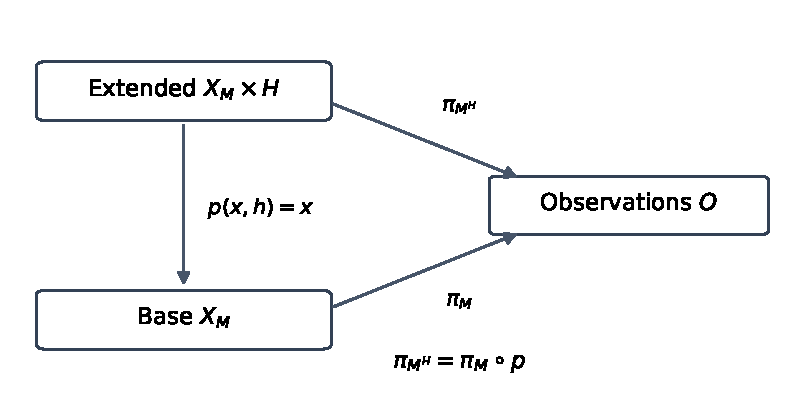
\includegraphics[width=0.84\textwidth]{figures/concept_hidden_extension.pdf}
\caption{Hidden factor extension and observation preserving projection. The projection is surjective. Distinct hidden values attached to one base state create distinct extended states with one common observation.}
\label{fig:hiddencover}
\end{figure}

\begin{theorem}[Hidden extensions preserve empirical equivalence]
For every inhabited \(H\),
\[
\Obs(\Model^H)=\Obs(\Model).
\]
Therefore \(\Model^H\approx\Model\).
\end{theorem}

\begin{proof}
Every extended observation has the form \(\pi_{\Model^H}(x,h)=\pi_\Model(x)\), so \(\Obs(\Model^H)\subseteq\Obs(\Model)\). Conversely, choose an anchor \(h_0\in H\). For every \(x\in X_\Model\), the extended state \((x,h_0)\) produces \(\pi_\Model(x)\). Hence \(\Obs(\Model)\subseteq\Obs(\Model^H)\).
\end{proof}
\begin{corollary}[Experimental invariance of hidden extensions]
For every admissible experiment \(e\),
\[
\Out_e(\Model^H)=\Out_e(\Model).
\]
\end{corollary}
\begin{theorem}[Hidden collisions]
If \(H\) contains distinct values \(h_0\neq h_1\) and \(X_\Model\) contains \(x\), then
\[
(x,h_0)\neq(x,h_1)
\]
but
\[
\pi_{\Model^H}(x,h_0)=\pi_{\Model^H}(x,h_1).
\]
Therefore the extended observation map is noninjective and \(\Model^H\) has no exact latent decoder.
\end{theorem}

\begin{proof}
The ordered pairs are distinct because their second coordinates differ. Both observations reduce by definition to \(\pi_\Model(x)\). The observation map is therefore noninjective. Exact latent decoding would imply injectivity, which is impossible.
\end{proof}
The Boolean extension uses \(H=\bool\). The duplicate model is the same two copy construction written as a specific finite hidden factor.

\subsection{Finite hidden multiplicity}

For a positive integer \(m\), define
\[
X_{\Model^{(m)}}=X_\Model\times\{0,1,\ldots,m-1\}
\]
and ignore the second coordinate during observation. Each base latent state generates \(m\) extended states in one observation fiber.

\begin{proposition}[Arbitrary finite hidden families]
For every base state \(x\in X_\Model\), the map
\[
\iota_x:\{0,\ldots,m-1\}\to X_{\Model^{(m)}},
\qquad
\iota_x(j)=(x,j),
\]
is injective, and every state in its image produces \(\pi_\Model(x)\).
\end{proposition}
Thus finite latent multiplicity can be increased without changing reachable observations or any admissible outcome set. In the verified source, \texttt{finiteMultiplicityModel M n} uses the hidden type \(\operatorname{Fin}(n+1)\); the paper parameter \(m\) is therefore \(n+1\).

\subsection{Countable hidden multiplicity}

The construction is not restricted to finite hidden sets. Let
\[
X_{\Model^{(\mathbb N)}}=X_\Model\times\mathbb N
\]
and define
\[
\pi_{\Model^{(\mathbb N)}}(x,n)=\pi_\Model(x).
\]
For each \(x\), the map \(n\mapsto(x,n)\) embeds \(\mathbb N\) into the observation fiber over \(\pi_\Model(x)\). The model remains empirically equivalent to \(\Model\), and every admissible outcome set remains equal. If \(X_\Model\neq\varnothing\), distinct natural number coordinates give a collision, so exact latent decoding is impossible.

This result separates empirical class size from latent fiber size. An empirical class can contain representatives with one, finitely many, or countably many latent states above the same accessible observation.

\subsection{Latent covers}

The product construction is one example of a more general relation.

\begin{definition}[Latent cover]
An extended model \(\Extended\) is a latent cover of a base model \(\Model\) when there exists a surjective projection
\[
p:X_{\Extended}\to X_\Model
\]
such that
\[
\pi_{\Extended}(z)=\pi_\Model(p(z))
\]
for every \(z\in X_{\Extended}\).
\end{definition}
Latent covers compose. The identity map makes each model a cover of itself.

\begin{theorem}[A latent cover is empirically equivalent to its base]
If \(\Extended\) covers \(\Model\), then
\[
\Obs(\Extended)=\Obs(\Model).
\]
Consequently, every admissible experiment has the same possible outcomes under both models.
\end{theorem}

\begin{proof}
Observation preservation shows that every observation of \(\Extended\) is an observation of \(\Model\). Surjectivity shows that every base latent state has an extended preimage, and observation preservation gives the same accessible output. Hence the reachable sets are equal. Outcome equality follows from \Cref{thm:outcomeinvariance}.
\end{proof}
\begin{definition}[Strict latent cover]
A latent cover is strict when its projection \(p\) is noninjective.
\end{definition}
A strict cover contains distinct extended states that project to one base state. Observation preservation then forces those extended states to share one observation.

\begin{theorem}[Strict covers prevent exact latent reconstruction]
If \(\Extended\) is a strict latent cover of \(\Model\), then \(\pi_{\Extended}\) is noninjective and \(\Extended\) has no exact latent decoder.
\end{theorem}

\begin{proof}
Since the projection is noninjective, choose \(z_1\neq z_2\) with \(p(z_1)=p(z_2)\). Observation preservation gives
\[
\pi_{\Extended}(z_1)
=\pi_\Model(p(z_1))
=\pi_\Model(p(z_2))
=\pi_{\Extended}(z_2).
\]
Thus the extended observation map is noninjective. Exact decoding is therefore impossible.
\end{proof}
\subsection{Existence of strict covers for inhabited models}

Every inhabited model has a Boolean strict hidden extension. The construction can then be repeated.

\begin{theorem}[Every inhabited model admits a strict latent cover]
For every generative model with at least one latent state, there exists an empirically equivalent strict latent cover with additional latent distinctions.
\end{theorem}

\begin{proof}
Use the Boolean hidden extension. Projection onto the base state is surjective and observation preserving. The two Boolean values make the projection noninjective.
\end{proof}
The Lean predicate \texttt{LatentlyMaximal} means that no strict latent cover exists. The theorem negates that predicate for every inhabited model. This definition is not ordinary maximality in a partial order. A strict cover means a noninjective surjective projection; for infinite models such a projection may be a self-map. For example, \(X=\mathbb N\), \(O=\{0\}\), and \(\pi(n)=0\) admit the strict self-cover \(p(n)=\lfloor n/2\rfloor\). Surjectivity follows from \(p(2n)=n\), and \(p(0)=p(1)\) proves noninjectivity. Additional hidden labels also need not increase an infinite set's cardinality. The proved conclusion is the existence of strict covers within the specified model class. It does not assert a physically realized hierarchy of hidden variables.

\section{The empirical model quotient}
\label{sec:empiricalquotient}

Empirical equivalence partitions generative models into classes with equal reachable observation sets. The empirical model quotient records only this accessible information. The descent results use the same representative-independence principle as ordinary quotient constructions and universal properties \parencite{MacLaneBirkhoff1999,Leinster2014}, now applied to a space of models.

\begin{definition}[Empirical model quotient]
Let \(\mathfrak M_O\) denote the collection of generative models over \(O\), with a fixed set theoretic universe for latent spaces. The Lean development makes the corresponding universe parameters explicit. The empirical model quotient is
\[
\mathfrak M_O/{\approx},
\]
where \(\Model\approx\Model'\) means \(\Obs(\Model)=\Obs(\Model')\).
\end{definition}
The canonical projection sends each model to its empirical class:
\[
q_{\Emp}:\mathfrak M_O\to\mathfrak M_O/{\approx}.
\]
Two canonical classes are equal exactly when the corresponding models are empirically equivalent.

\subsection{Invariant properties descend}

\begin{theorem}[Universal property for model properties]
A property \(P:\mathfrak M_O\to\{\mathrm{false},\mathrm{true}\}\) is observation invariant if and only if there exists a unique property
\[
\bar P:\mathfrak M_O/{\approx}\to\{\mathrm{false},\mathrm{true}\}
\]
such that
\[
P=\bar P\circ q_{\Emp}.
\]
\end{theorem}

\begin{proof}
If \(P\) is observation invariant, define \(\bar P([\Model])=P(\Model)\). This is well defined because all representatives of one class have the same truth value. The factorization follows from the definition, and uniqueness follows because every quotient class has a representative. Conversely, any property factored through the quotient is constant on each quotient class and is therefore observation invariant.
\end{proof}
The same result holds for arbitrary valued measurements.

\begin{theorem}[Universal property for invariant measurements]
Let \(F:\mathfrak M_O\to V\). The map \(F\) assigns equal values to empirically equivalent models if and only if there exists a unique
\[
\bar F:\mathfrak M_O/{\approx}\to V
\]
such that \(F=\bar F\circ q_{\Emp}\).
\end{theorem}
\begin{figure}[tbp]
\centering
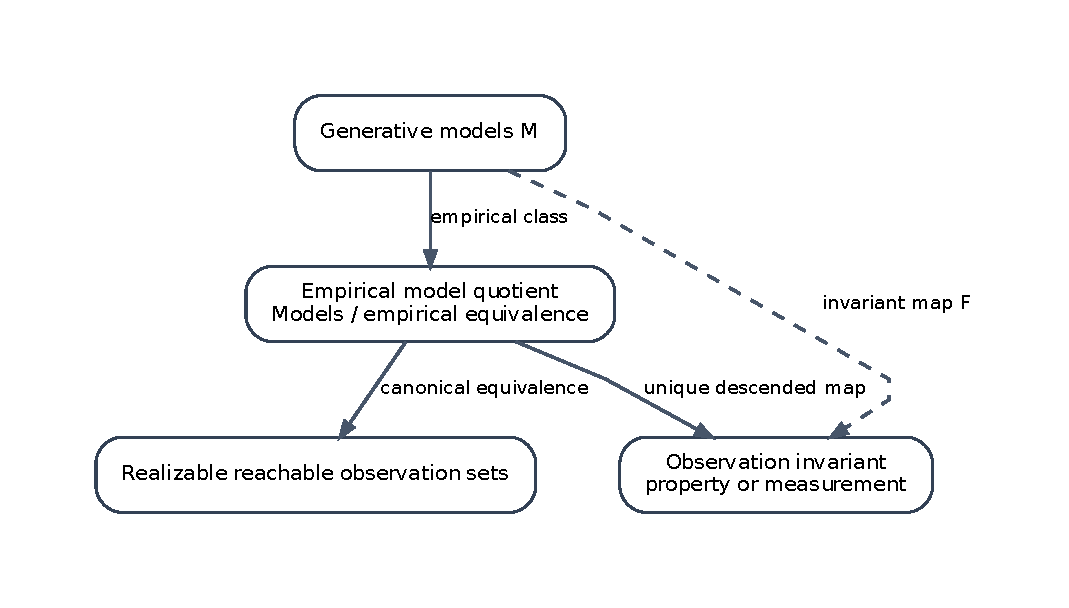
\includegraphics[width=0.86\textwidth]{figures/concept_empirical_quotient.pdf}
\caption{Empirical quotient and invariant descent. Observation invariant properties and measurements factor uniquely through empirical classes. Exact latent reconstructability fails this condition because it varies among representatives of one class.}
\label{fig:empiricalquotient}
\end{figure}

\subsection{Realizable observation sets}

The quotient has a concrete representation.

\begin{definition}[Realizable observation set]
A subset \(A\subseteq O\) is realizable when there exists a generative model \(\Model\) such that
\[
\Obs(\Model)=A.
\]
\end{definition}
\begin{theorem}[Canonical representation of empirical classes]
The map
\[
[\Model]\longmapsto\Obs(\Model)
\]
is a bijection between the empirical model quotient and the collection of realizable reachable observation sets.
\end{theorem}

\begin{proof}
The map is well defined because empirically equivalent models have equal reachable sets. It is injective because equal reachable sets imply empirical equivalence and therefore equal quotient classes. It is surjective by the definition of realizability.
\end{proof}
Each empirical class therefore specifies one reachable set. Whether a latent property is fixed within that class depends on the allowed models. For example, an empty reachable set forces an empty latent space.

\subsection{Exact reconstruction does not descend}

\begin{theorem}[Exact latent reconstruction is not a quotient property]
Assume \(O\neq\varnothing\) and a model class containing \((O,\id_O)\) and its Boolean hidden extension. Exact latent reconstructability does not factor through the empirical model quotient of that class.
\label{thm:decoderdoesnotdescend}
\end{theorem}

\begin{proof}
Use the identity model on \(O\); it is inhabited and has the identity decoder. Its Boolean hidden extension is empirically equivalent to the base. The extension has a noninjective observation map and no exact latent decoder. Therefore the property has different truth values on two representatives of one empirical class. A property with that variation cannot descend to the quotient.
\end{proof}
The identity model gives a counterexample at the full observation space. An inclusion map gives a counterexample at any prescribed nonempty reachable set.

\begin{corollary}[Decoder status at a prescribed reachable set]
Let \(\varnothing\ne S\subseteq O\). If the model class contains the inclusion \(i:S\hookrightarrow O\) and its Boolean extension, the empirical class for \(S\) contains both an exactly decodable model and one without a decoder. If the reachable set is empty, all compatible models have the same decoder status.
\end{corollary}

\begin{proof}
Choose \(s_0\in S\). The map \(d:O\to S\) that returns \(o\) for \(o\in S\) and \(s_0\) otherwise satisfies \(d\circ i=\id_S\). Its Boolean extension reaches the same set, and \((s_0,0)\) and \((s_0,1)\) prevent exact decoding. If the reachable set is empty, a source state would give a reachable value, so the source is empty. A total map from \(O\) into the empty set exists precisely when \(O\) is empty.
\end{proof}

\section{Synthesis theorem}
\label{sec:synthesis}

Every model with a nonempty state space has a strict hidden extension that preserves all reachable outputs and prevents exact recovery of the extended state.

\begin{theorem}[Boundary limited observer synthesis]
Let \(\Model=(X_\Model,\pi_\Model)\) be a generative model, let \(x_0\in X_\Model\) be an inhabited witness, and let \(e:O\to R\) be an admissible experiment. Then there exists a model \(\Extended\) such that:
\begin{enumerate}[label=(\roman*)]
\item \(\Extended\) is a strict latent cover of \(\Model\);
\item the empirical classes are equal, \(q_{\Emp}(\Extended)=q_{\Emp}(\Model)\), equivalently \(\Extended\approx\Model\);
\item \(\Obs(\Extended)=\Obs(\Model)\);
\item \(\Out_e(\Extended)=\Out_e(\Model)\); and
\item \(\Extended\) has no exact latent decoder.
\end{enumerate}
\label{thm:synthesis}
\end{theorem}

\begin{proof}
Choose the Boolean extension
\[
X_{\Extended}=X_\Model\times\bool
\]
and define
\[
\pi_{\Extended}(x,b)=\pi_\Model(x).
\]
Define the projection
\[
p:X_{\Extended}\to X_\Model,
\qquad
p(x,b)=x.
\]
The projection is surjective. For each \(x\in X_\Model\), the state \((x,0)\) maps to \(x\). It also preserves observation because
\[
\pi_{\Extended}(x,b)=\pi_\Model(p(x,b)).
\]
Thus \(\Extended\) is a latent cover of \(\Model\).

The cover is strict. Use the supplied witness \(x_0\in X_\Model\). Then
\[
(x_0,0)\neq(x_0,1)
\]
but
\[
p(x_0,0)=x_0=p(x_0,1).
\]
Hence the projection is noninjective.

Every latent cover is empirically equivalent to its base. Therefore
\[
\Extended\approx\Model
\]
and
\[
\Obs(\Extended)=\Obs(\Model).
\]
By empirical outcome invariance,
\[
\Out_e(\Extended)=\Out_e(\Model).
\]
Finally, the two distinct extended states \((x_0,0)\) and \((x_0,1)\) have equal observations:
\[
\pi_{\Extended}(x_0,0)=\pi_\Model(x_0)=\pi_{\Extended}(x_0,1).
\]
The extended observation map is noninjective. An exact latent decoder would imply injectivity. Therefore no exact latent decoder exists for \(\Extended\).
\end{proof}
\begin{figure}[tbp]
\centering
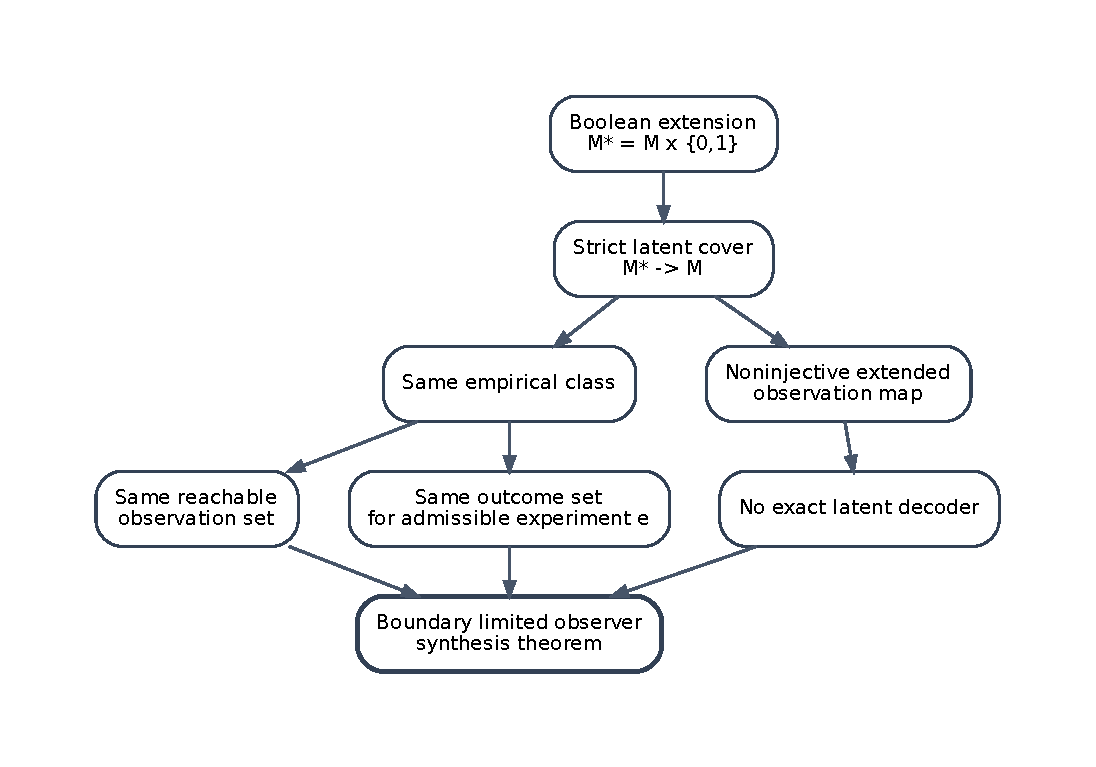
\includegraphics[width=0.82\textwidth]{figures/concept_synthesis_dependency.pdf}
\caption{Dependency structure of the synthesis theorem. The result combines fiber based reconstruction limits, model outcome invariance, strict hidden extensions, and empirical quotient structure.}
\label{fig:dependency}
\end{figure}

\subsection{Recovery from possible outputs}

The extension and its base agree on the entire reachable set. Every function of the observation, including the identity, gives the same possible outcomes. The extension always lacks an exact decoder. The base may admit one.

Uniqueness of a latent representation requires a restriction on the admissible models or a further measurement. Dynamics, causal interventions, regularity, minimality, prior probabilities, and known state counts give different restrictions. Their justification depends on the application.

\subsection{Physical interpretation}

The Boolean label provides a second representation consistent with the same outputs. A physical interpretation of that label requires independent evidence. Approximate reconstruction would require a loss function, and probabilistic reconstruction would require a law on states or observations. A refined measurement would define a new equivalence relation.

\section{Assumption checks and counterexamples}
\label{app:scopechecks}
These examples establish the qualifications used in the main text. They are elementary derivations and executable regression cases, not additions to the pinned Lean formalization.

\subsection{Reachable collisions in a composite map}
Let \(f:\{0,1\}\to\{0,1,2\}\) satisfy \(f(0)=0\), \(f(1)=1\). Let \(g(0)=0\), \(g(1)=g(2)=1\). The map \(g\) is noninjective, but \(g\circ f=\id_{\{0,1\}}\). Its collision lies outside the restriction of \(g\) to the reachable set \(f[X]\). Conversely, if distinct original states satisfy \(f(x)=f(y)\), then \(g(f(x))=g(f(y))\) for every downstream function \(g\). This proves the corrected composition statement.

\subsection{Decoder status of an already noninjective base}
Take \(X=\{0,1\}\), \(O=\{0\}\), and \(\pi(x)=0\). No exact decoder exists. Its Boolean extension also has a constant observation map and no decoder. Thus the extension theorem guarantees failure of decoding for the extension, while a change of decoder status additionally requires a decodable base.

\subsection{Empty spaces and total decoders}
If \(O=\varnothing\), existence of \(\pi:X\to O\) forces \(X=\varnothing\). The empty decoder is a left inverse. If \(X=\varnothing\) but \(O\neq\varnothing\), no total map \(d:O\to X\) exists, although \(\pi\) is injective. If \(X\neq\varnothing\) and \(\pi\) is injective, fix \(x_0\in X\). Define \(d(o)\) as the unique preimage for reachable \(o\), and as \(x_0\) otherwise. Then \(d\circ\pi=\id_X\). These cases justify the exact-decoder condition and the nonempty assumption in the global nonidentifiability theorems.

\subsection{Equal possible outputs and different probability laws}
For \(0<p<1\), the Bernoulli law has reachable outcomes \(\{0,1\}\). In particular, \(p=1/10\) and \(p=9/10\) share this set but differ in \(\Pr(Y=1)\). Any extension of empirical equivalence to statistical experiments must include the probability law. Equality of reachable sets alone supplies no statement about equal frequencies or likelihoods.

\subsection{Temporal reconstruction and conditioning}
For \(\dot x_1=x_2\), \(\dot x_2=0\), and \(y=x_1\), the exact solution is
\[
y(t)=x_1(0)+t x_2(0).
\]
At time zero, all values of \(x_2(0)\) share one output for a fixed \(x_1(0)\). The two-sample map is
\[
\begin{pmatrix}y(0)\\y(T)\end{pmatrix}
=\begin{pmatrix}1&0\\1&T\end{pmatrix}
\begin{pmatrix}x_1(0)\\x_2(0)\end{pmatrix}.
\]
Its determinant is \(T\), so it is invertible when \(T\neq0\), with
\[
x_1(0)=y(0),\qquad x_2(0)=\frac{y(T)-y(0)}{T}.
\]
If the two output errors are bounded by \(\eta\), the recovered \(x_2\) error is at most \(2\eta/|T|\). Opposite signed endpoint errors attain the bound. Invertibility alone therefore gives no uniform stability as \(T\to0\). The regression test uses rational arithmetic, so it checks the exact formulas without integration or floating point tolerances.

\section{Computational methods}
\label{sec:computationalmethods}

The calculation enumerates the latent states, outputs, and pairs of states in each finite model.

\subsection{Implementation and reproducibility}

The Python program evaluates each processing rule on every reachable observation. It also computes the observation fibers and the refinement maps. The supplement includes source excerpts and the filenames of the complete records.

\begin{table}[tbp]
\centering
\caption{Computational outputs used in the finite study.}
\label{tab:computationaloutputs}
\small
\begin{tabularx}{\textwidth}{@{}lX@{}}
\toprule
Output group & Contents \\
\midrule
Model summaries & Latent counts, reachable observations, fiber statistics, collision counts, injectivity, exact decoder status, and hidden multiplicity. \\
Experiment summaries & Possible outcome sets and equality with the injective base for four observation only experiments. \\
Predicate summaries & Existential success profiles and complete finite truth profiles for three accessible predicates. \\
Empirical quotient & Grouping of models by equality of reachable observation sets and comparison of latent properties within one class. \\
Refinement summaries & Interface sizes, strictness, collapsed pairs, reverse refinement, and induced quotient map properties. \\
Validation & Tests of the reference implementation, scope conditions, and measurement criteria. \\
\bottomrule
\end{tabularx}
\end{table}

\subsection{Finite models, fibers, and collision counts}

The finite models use integer observation labels. We compare their reachable sets in the common space \(O=\{0,1,2,3,4,5\}\), including the modulo-three outputs \(0,1,2\) by their usual inclusion. The primary model has latent states
\[
X=\{0,1,2,3,4,5\}
\]
and the identity observation map. A comparison model uses the same latent states and the rule \(\pi(x)=x\bmod 3\). For every reachable observation \(o\), the implementation enumerates the fiber
\[
F_o=\pi^{-1}(o)
\]
and calculates the unordered collision count
\[
C(\Model)=\sum_{o\in\Obs(\Model)}\binom{|F_o|}{2}.
\]
This sum counts unordered pairs of distinct states with the same observation.

\subsection{Hidden multiplicity family}

The Boolean extension attaches \(\{\mathrm{false},\mathrm{true}\}\) to each base state and ignores the added coordinate during observation. The finite family attaches
\[
H_m=\{0,1,\ldots,m-1\},
\qquad
m\in\{1,2,3,5,8\},
\]
with observation rule
\[
\pi_m(x,h)=x.
\]
For the six state injective base, the finite identities are
\[
|X_m|=6m,
\qquad
|\Obs(\Model_m)|=6,
\qquad
|F_o|=m,
\qquad
C(\Model_m)=6\binom{m}{2}=3m(m-1).
\]
An exact decoder exists in this family only for \(m=1\).

\subsection{Observation only experiments and predicates}

Four rules process the observation: identity, a threshold at three, a partition into three categories, and a partition into bins of width two. Each rule acts on every reachable output.

The three predicates test evenness, \(o\geq 3\), and membership in \(\{0,5\}\). The existential profile records whether each predicate succeeds for at least one output. The truth table records its value on every reachable output.

\subsection{Finite empirical quotient and interface refinement}

The finite empirical quotient groups models by exact equality of reachable observation sets. The grouping rule does not compare latent cardinality, fiber size, decoder status, or hidden factor metadata.

The refinement study uses one eight state world and four interfaces: identity, paired buckets, binary regions, and a relabeled identity. Each proposed refinement is checked on every world state. The implementation then records strictness, collapsed state pairs, reverse refinement, equality of observational resolution, and surjectivity, injectivity, and bijectivity of the induced finite quotient map.

\subsection{Automated validation}

The reference implementation has eighteen tests. Six further tests check assumptions about composition, decoding, probability, and temporal records. Two tests enumerate all reachable sets in codomains of size zero through three and all 4,096 triples of binary maps on four states. The suite also checks hidden extensions, predicate profiles, quotient grouping, reverse refinement, relabeling, and invalid coarsening. The program stops if any finite identity fails.


\subsection{Formal proofs and finite calculations}

Lean checks the proofs from the encoded definitions. Python enumerates the finite examples and checks each count against those definitions. The supplement identifies the Lean declarations and the source of the finite records.

Applying a proof to a physical device requires a model of its state, evolution, and readout \parencite{Horsman2014,Horsman2015}. Measurement noise, approximation error, and omitted variables affect that application.

\section{Computational results}
\label{sec:results}

The finite calculations satisfy the stated identities and invariance checks. The tables report exact enumerations, and the figures display the corresponding results for the multiplicity and refinement families.

\subsection{Base models and Boolean extension}

The injective base contains six latent states and six reachable observations. Every fiber has size one, the observation map is injective, and an exact decoder exists. The noninjective comparison contains six latent states and three reachable observations. Each reachable fiber has size two, the model contains three unordered latent collisions, and no exact decoder exists. The Boolean extension contains twelve latent states and the same six reachable observations as the injective base. Its maximum fiber size is two, it contains six collision pairs, and no exact decoder exists.

\begin{table}[tbp]
\centering
\caption{Base and Boolean extension calculations.}
\label{tab:baseboolean}
\small
\begin{tabular}{@{}lrrrrcc@{}}
\toprule
Model & Latent & Reachable & Max. fiber & Collisions & Injective & Exact decoder \\
\midrule
Injective base & 6 & 6 & 1 & 0 & True & True \\
Noninjective base & 6 & 3 & 2 & 3 & False & False \\
Boolean extension & 12 & 6 & 2 & 6 & False & False \\
\bottomrule
\end{tabular}
\end{table}

\subsection{Finite hidden multiplicity}

The latent state count increases linearly with hidden multiplicity. The reachable observation count remains fixed at six, and the maximum fiber size equals the hidden multiplicity. The four panels show the latent-state, reachable-observation, fiber-size, and experiment-outcome consequences of the same multiplicity construction.

\begin{figure}[tbp]
\centering
\begin{subfigure}[t]{0.49\textwidth}
\centering
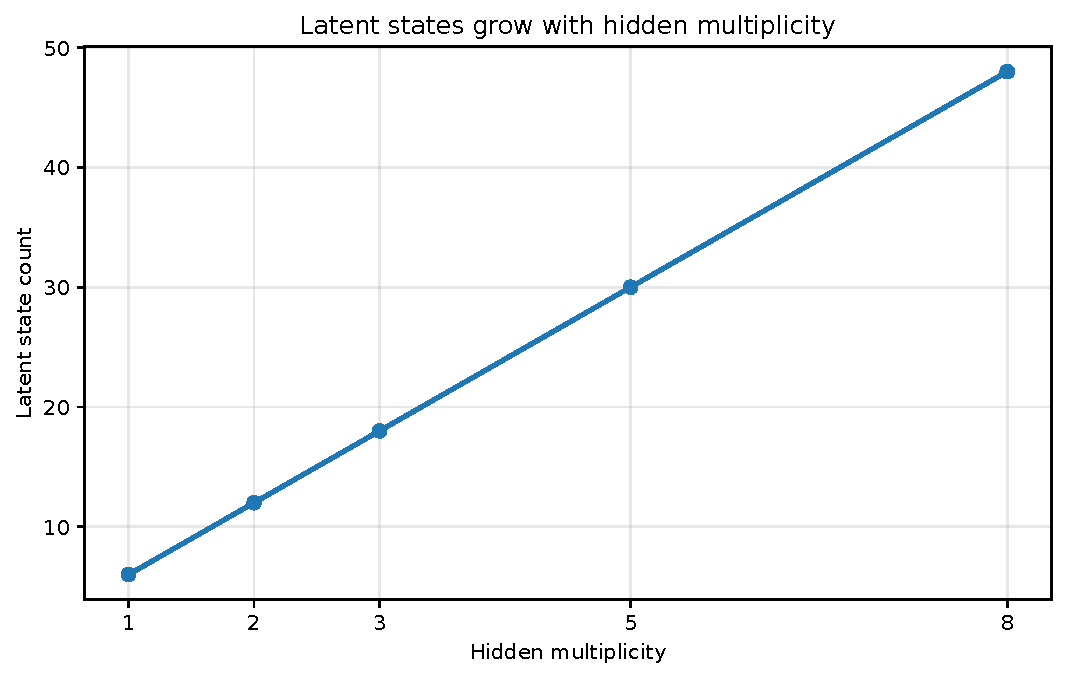
\includegraphics[width=\linewidth]{figures/repo_latent_state_count_vs_hidden_multiplicity.pdf}
\caption{Latent state count.}
\label{fig:repo-latent}
\end{subfigure}\hfill
\begin{subfigure}[t]{0.49\textwidth}
\centering
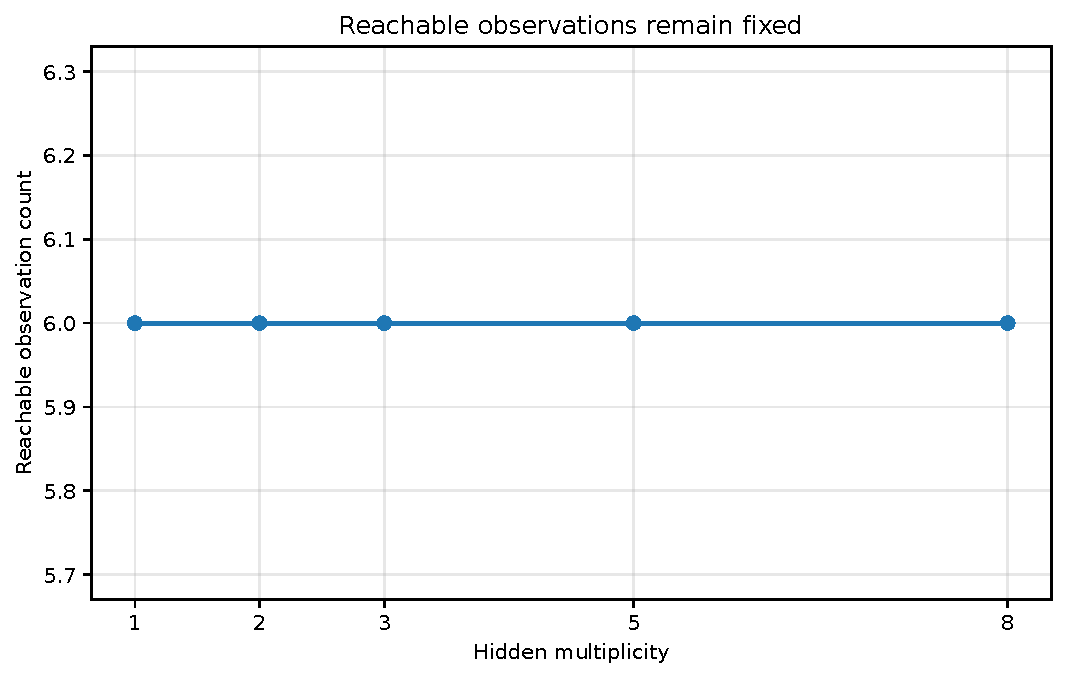
\includegraphics[width=\linewidth]{figures/repo_reachable_observation_count_vs_hidden_multiplicity.pdf}
\caption{Reachable observation count.}
\label{fig:repo-reachable}
\end{subfigure}

\vspace{0.6em}
\begin{subfigure}[t]{0.49\textwidth}
\centering
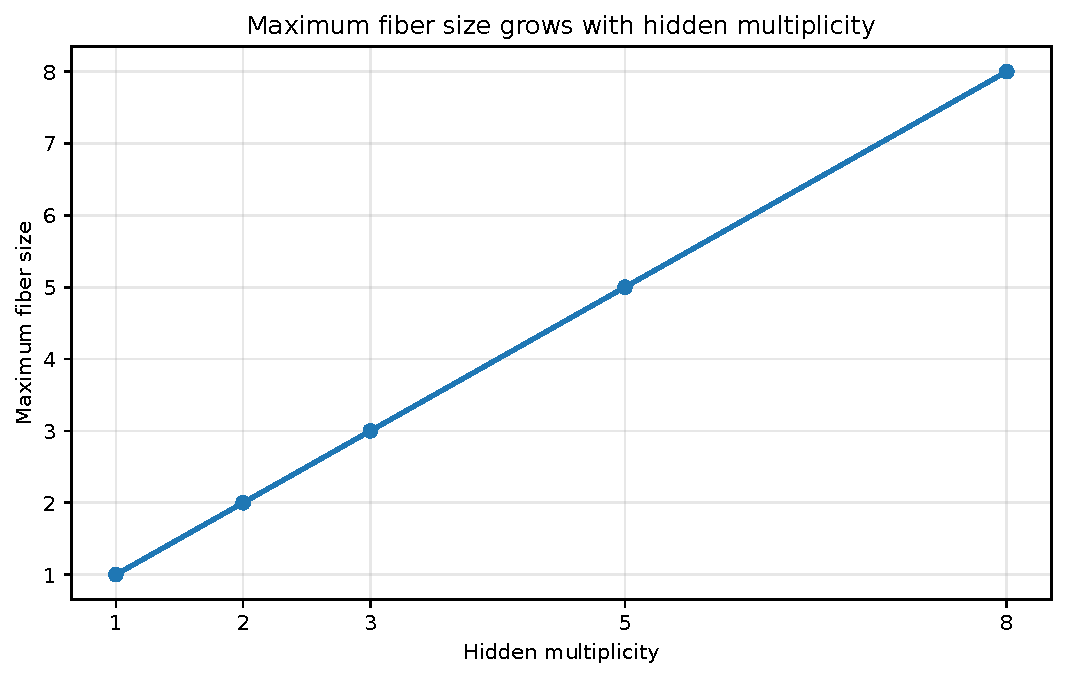
\includegraphics[width=\linewidth]{figures/repo_maximum_fiber_size_vs_hidden_multiplicity.pdf}
\caption{Maximum fiber size.}
\label{fig:repo-fiber}
\end{subfigure}\hfill
\begin{subfigure}[t]{0.49\textwidth}
\centering
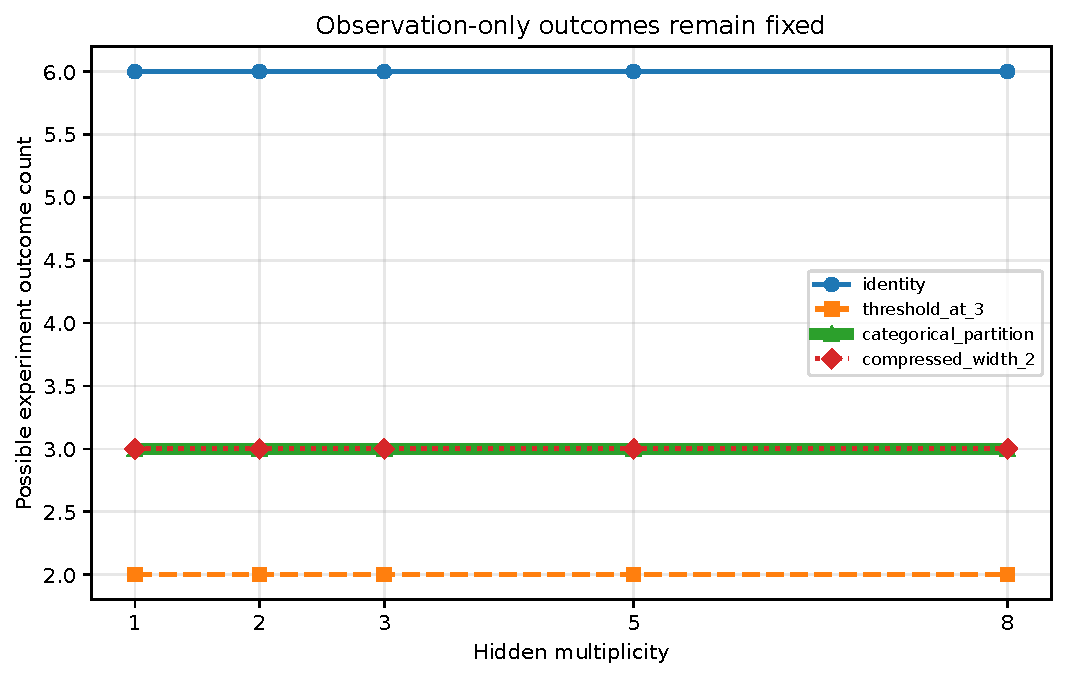
\includegraphics[width=\linewidth]{figures/repo_experiment_outcome_count_vs_hidden_multiplicity.pdf}
\caption{Observation only outcome counts.}
\label{fig:repo-experiments}
\end{subfigure}
\caption{Hidden multiplicity and observation only experiment results. The latent representation and observation fibers grow while the reachable observation set and each experiment's possible outcome count remain fixed.}
\label{fig:multiplicitypanel}
\end{figure}

\begin{table}[tbp]
\centering
\caption{Complete finite multiplicity summary.}
\label{tab:multiplicity}
\small
\begin{tabular}{@{}rrrrrrl@{}}
\toprule
\(m\) & Latent & Reachable & Avg. fiber & Max. fiber & Collisions & Exact decoder \\
\midrule
1 & 6 & 6 & 1.00 & 1 & 0 & True \\
2 & 12 & 6 & 2.00 & 2 & 6 & False \\
3 & 18 & 6 & 3.00 & 3 & 18 & False \\
5 & 30 & 6 & 5.00 & 5 & 60 & False \\
8 & 48 & 6 & 8.00 & 8 & 168 & False \\
\bottomrule
\end{tabular}
\end{table}

Every row is marked empirically equivalent to the base. Latent cardinality, fiber size, collision count, injectivity, and exact decoder status change while the reachable observation set remains fixed.

\subsection{Observation only experiments and predicate profiles}

The identity experiment has six possible outcomes. The threshold experiment has two. The categorical partition and width two compression experiments each have three. All twenty eight model and experiment comparisons match the base outcome set for the corresponding experiment.

\begin{table}[tbp]
\centering
\caption{Observation only outcome sets.}
\label{tab:experiments}
\small
\begin{tabularx}{\textwidth}{@{}lXcc@{}}
\toprule
Experiment & Possible outcomes & Count & All listed models match base \\
\midrule
Identity & \(\{0,1,2,3,4,5\}\) & 6 & True \\
Threshold at three & \(\{\mathrm{false},\mathrm{true}\}\) & 2 & True \\
Categorical partition & \(\{\mathrm{high},\mathrm{low},\mathrm{middle}\}\) & 3 & True \\
Compression width two & \(\{0,1,2\}\) & 3 & True \\
\bottomrule
\end{tabularx}
\end{table}

Three predicates are evaluated for seven model representations. All twenty one existential comparisons match the base success profile. All twenty one complete truth profile comparisons also match the base.

\begin{table}[tbp]
\centering
\caption{Base predicate profiles and comparison counts.}
\label{tab:predicates}
\small
\begin{tabularx}{\textwidth}{@{}lXcc@{}}
\toprule
Predicate & Base truth table on \(0,\ldots,5\) & Models compared & Matches \\
\midrule
Even & T, F, T, F, T, F & 7 & 7 \\
At least three & F, F, F, T, T, T & 7 & 7 \\
Endpoint \(\{0,5\}\) & T, F, F, F, F, T & 7 & 7 \\
\bottomrule
\end{tabularx}
\end{table}

\subsection{Finite empirical quotient and varying latent properties}

The finite grouping procedure produces two empirical classes. The first contains the injective base, Boolean extension, and finite multiplicity extensions. Its reachable set is \(\{0,1,2,3,4,5\}\), while its representatives have latent cardinalities \(6,12,18,30,48\). The second contains the noninjective comparison model with reachable set \(\{0,1,2\}\).

\begin{table}[tbp]
\centering
\caption{Finite empirical quotient.}
\label{tab:empiricalclasses}
\small
\begin{tabularx}{\textwidth}{@{}cXlX@{}}
\toprule
Class & Reachable observation set & Latent cardinalities & Representative types \\
\midrule
1 & \(\{0,1,2,3,4,5\}\) & 6, 12, 18, 30, 48 & Base, Boolean, and finite multiplicity extensions \\
2 & \(\{0,1,2\}\) & 6 & Noninjective comparison model \\
\bottomrule
\end{tabularx}
\end{table}

Four latent properties vary between the injective base and its Boolean extension although the two models occupy the same finite empirical class.

\begin{table}[tbp]
\centering
\caption{Properties that vary inside one finite empirical class.}
\label{tab:nonidentifiable}
\small
\begin{tabularx}{\textwidth}{@{}Xccc@{}}
\toprule
Property & Base & Boolean extension & Varies \\
\midrule
Latent cardinality & 6 & 12 & True \\
Maximum observation fiber size & 1 & 2 & True \\
Existence of exact latent decoder & True & False & True \\
Presence of Boolean hidden factor & False & True & True \\
\bottomrule
\end{tabularx}
\end{table}



\subsection{Interface refinement and quotient maps}

The identity and relabeled identity interfaces retain eight observable classes. Paired buckets retain four. Binary regions retain two. The strict refinements collapse four, eight, and twelve world state pairs. Their quotient maps are surjective and noninjective, and no reverse refinement exists. The relabeling maps collapse no pairs and induce bijections.

\begin{figure}[tbp]
\centering
\begin{subfigure}[t]{0.49\textwidth}
\centering
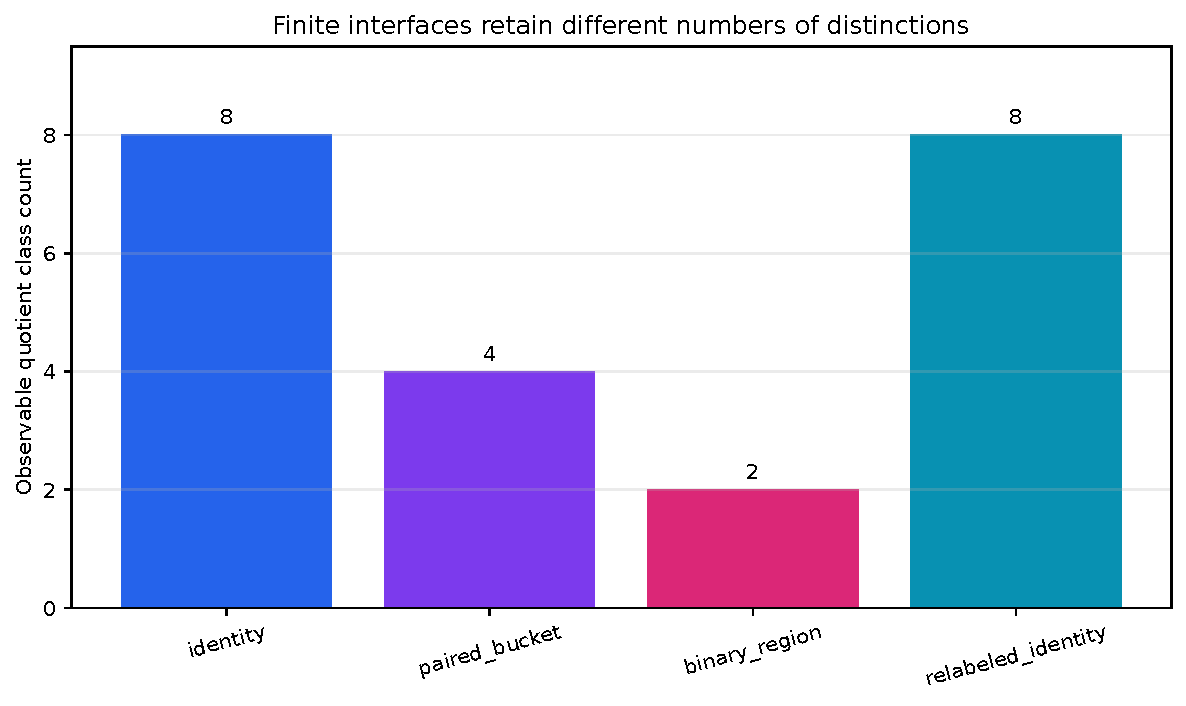
\includegraphics[width=\linewidth]{figures/repo_observable_quotient_size_by_interface.pdf}
\caption{Observable quotient size.}
\label{fig:repo-quotientsize}
\end{subfigure}\hfill
\begin{subfigure}[t]{0.49\textwidth}
\centering
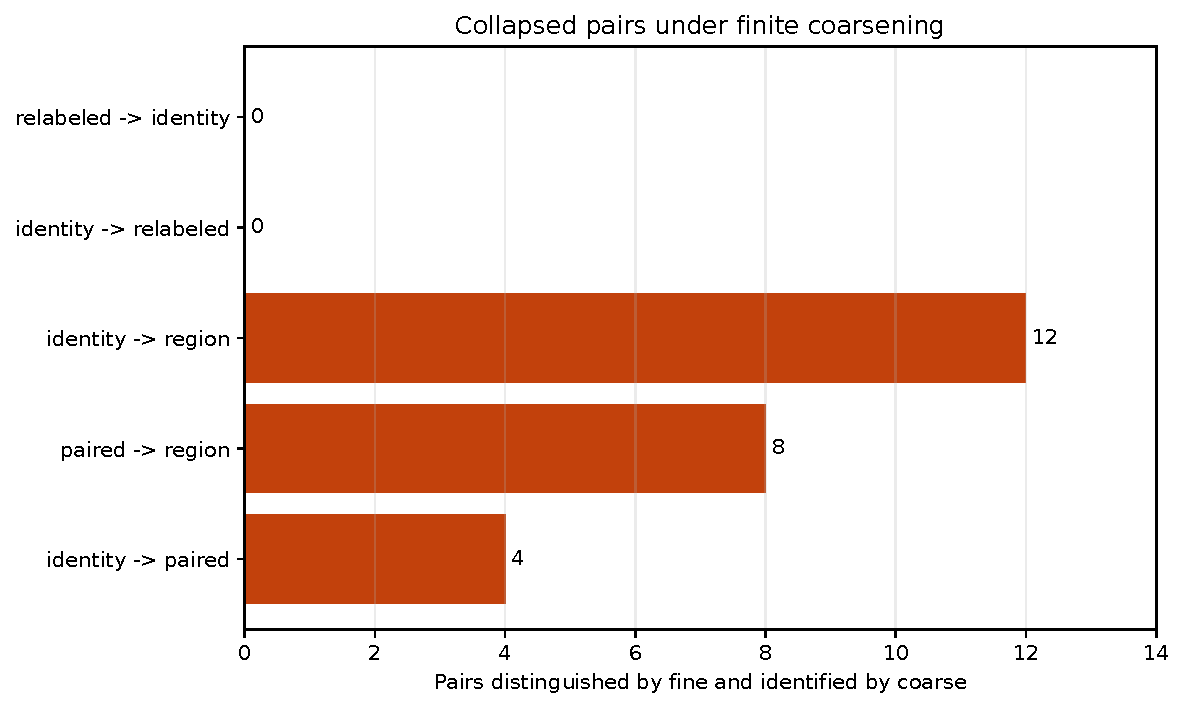
\includegraphics[width=\linewidth]{figures/repo_collapsed_pairs_by_refinement.pdf}
\caption{Collapsed state pairs.}
\label{fig:repo-collapsed}
\end{subfigure}
\caption{Interface refinement results. Strict coarsening reduces the retained quotient classes and identifies world state pairs. Relabeling preserves observational resolution.}
\label{fig:refinementpanel}
\end{figure}

\begin{table}[tbp]
\centering
\caption{Finite interface and refinement summary.}
\label{tab:refinements}
\small
\begin{tabularx}{\textwidth}{@{}Xrrrrcc@{}}
\toprule
Refinement & Fine \(Q\) & Coarse \(Q\) & Collapsed & Strict & Surjective & Injective \\
\midrule
Identity to paired & 8 & 4 & 4 & True & True & False \\
Paired to region & 4 & 2 & 8 & True & True & False \\
Identity to region & 8 & 2 & 12 & True & True & False \\
Identity to relabeled & 8 & 8 & 0 & False & True & True \\
Relabeled to identity & 8 & 8 & 0 & False & True & True \\
\bottomrule
\end{tabularx}
\end{table}

The files \nolinkurl{quotient_maps.csv} and \nolinkurl{collapsed_pairs.csv} contain the 36 entries in the quotient maps and the 24 collapsed pairs, respectively.

\subsection{Validation result}

All eighteen reference tests and eight additional finite checks pass. Each of the twelve regenerated CSV files matches its archived counterpart byte for byte.

\section{Operational architecture}
\label{sec:architecture}


\subsection{Process, feedback, and perspectival description}

The architecture is intentionally process-based. Whitehead's process philosophy is a historical precedent for treating events, transitions, and relations as primary descriptive units rather than reducing the analysis to static substances \parencite{Whitehead1978}. Wiener's cybernetics supplies the explicit language of feedback, communication, and control \parencite{Wiener1948}. Von Neumann's analyses of measurement and self-reproducing automata show why an observer, apparatus, description, and update rule cannot always be treated as independent endpoints \parencite{VonNeumann1955,VonNeumann1966}. Leibnizian perspectivism provides an earlier comparison for the idea that one world may admit multiple internally coherent representations \parencite{Leibniz1989}. None of these sources is identical to the map developed below. They explain why the complete object is a recursive transformation system rather than a single passive observation.

Bohm's distinction between implicate and explicate order and the Bohm--Hiley account of undivided quantum process are retained as comparative physical programs, not as assumptions of the present analysis \parencite{Bohm1980,BohmHiley1993}. The present theory requires only declared maps and equivalence relations. It does not infer an implicate order, a quantum ontology, or a universal process metaphysics from noninjectivity.

\subsection{The complete recursive scientific cycle}

The formal theory is a local core inside a larger scientific cycle. Let \(S(t)\) denote a physical or modeled state at time \(t\). Let \(A_i\) denote an apparatus, intervention, or sampling procedure. Let \(E_i\) denote a finite encoding or reconstruction step. Let \(O_i\) denote the representation accessible to an observer. Let \(L_i\) denote a reportable model, estimate, or claim. Let \(P_i\) denote a prediction, intervention, or next experimental choice. One cycle has the form
\[
S(t)
\longrightarrow A_i
\longrightarrow E_i
\longrightarrow O_i
\longrightarrow L_i
\longrightarrow P_i
\longrightarrow S(t+\Delta t).
\]
The final state enters the next cycle through new measurement. The complete process is recursive. This perception-action-return structure is compatible with predictive-processing and active-inference accounts in which observations update a generative model and actions change subsequent observations \parencite{RaoBallard1999,Friston2010,Parr2022,Friston2025ScaleFree}.

\begin{figure}[tbp]
\centering
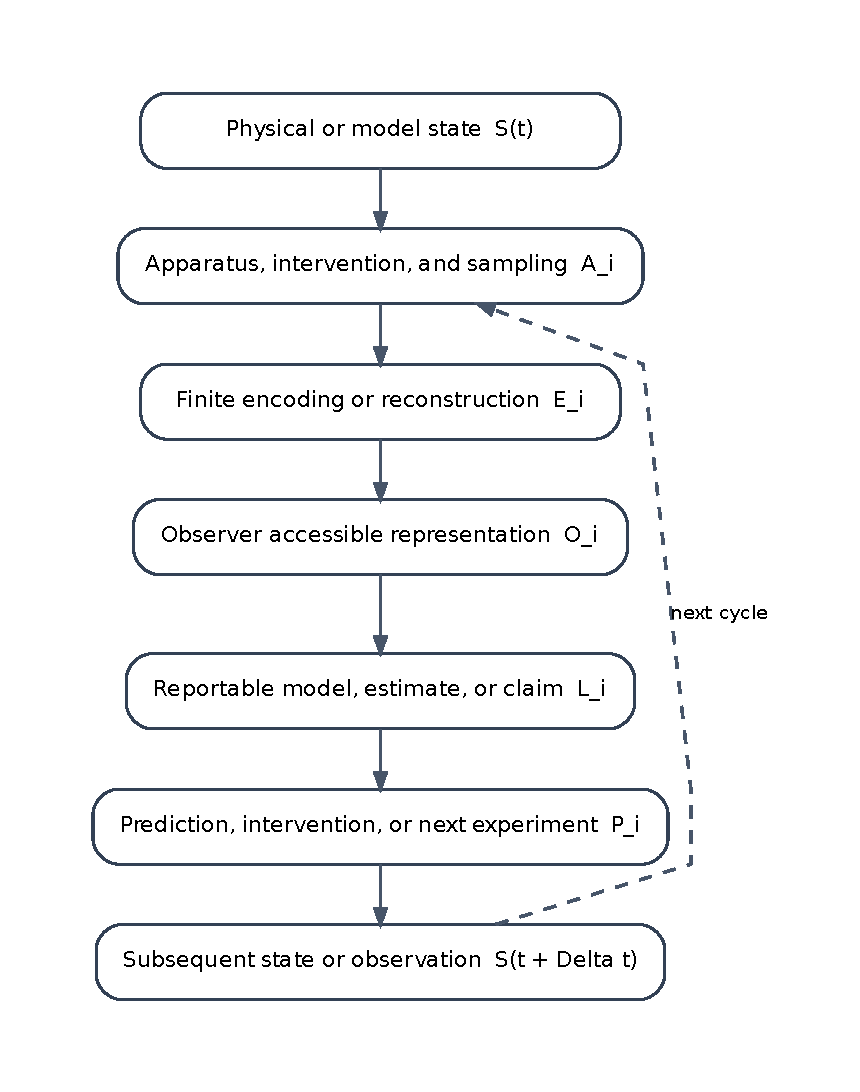
\includegraphics[height=0.67\textheight]{figures/concept_recursive_architecture.pdf}
\caption{Top-down scientific architecture. The map studied in this paper is the reduced local core of a longer recursive cycle. The dashed return marks prediction, intervention, and subsequent observation. The diagram is conceptual rather than a simulation output.}
\label{fig:recursivearchitecture}
\end{figure}

A physical state is not identical to an apparatus output. An apparatus output is not identical to a reconstructed feature. A reconstructed feature is not identical to an internal representation or report. A report is not identical to the next state of the system. Each arrow requires an explicit map.

\subsection{A distributed family of boundaries}

The complete route is better represented as a composition:
\[
X_{\mathrm{phys}}
\xrightarrow{\pi_{\mathrm{app}}}
O_{\mathrm{app}}
\xrightarrow{\pi_{\mathrm{bio}}}
O_{\mathrm{bio}}
\xrightarrow{\pi_{\mathrm{rep}}}
O_{\mathrm{rep}}
\xrightarrow{e}
R
\xrightarrow{a}
X'_{\mathrm{phys}}.
\]
The maps may correspond to physical coupling, detector response, sampling, reconstruction, biological sensing, attention, memory, language, or experimental decision. The aggregate observation map is
\[
\pi=\pi_{\mathrm{rep}}\circ\pi_{\mathrm{bio}}\circ\pi_{\mathrm{app}}.
\]
If two distinct original source states reach the same intermediate value, every subsequent deterministic map preserves that equality. The composite is then noninjective. Noninjectivity of a stage outside the range reached by preceding stages is insufficient; a counterexample is given in \Cref{app:scopechecks}. Refining a later report cannot recover a distinction that was already collapsed upstream unless new information enters through another route.

The stages should eventually be modeled separately rather than compressed into one aggregate map. Apparatus response, sampling, biological transduction, internal representation, report, and action may each preserve different relations and collapse different distinctions. Stage-specific models would show where a loss first occurs and whether later measurements introduce genuinely new information or only re-encode what has already passed through an earlier boundary.


\subsection{Computation as an interface-bound physical process}

A computation implemented in the world is not identical to its abstract description. It requires a physical encoding, a physical evolution, and a readout:
\[
S_{\mathrm{phys}}
\xrightarrow{\eta}
C
\xrightarrow{U}
C'
\xrightarrow{\rho}
R.
\]
Here \(\eta\) assigns an abstract computational state to a physical condition, \(U\) is the declared abstract evolution, and \(\rho\) converts a final physical or encoded state into a reportable result. Frameworks for physical computation make this representation relation explicit and distinguish the abstract calculation from the device that realizes it \parencite{Horsman2014,Horsman2015}. When the computation is embedded inside the system being studied, both \(\eta\) and \(\rho\) are themselves observer interfaces.

The distinction matters because different physical computers do not expose the same state space, elementary operations, error model, or readout. A digital computer represents finite symbolic states through engineered voltage ranges. An analog computer uses calibrated continuous physical variables to approximate a differential relation \parencite{Shannon1941}. A quantum computer manipulates quantum states but ultimately requires a controlled physical implementation and a classical measurement interface \parencite{DiVincenzo2000,AharonovCotlerQi2022}. A brain--computer interface converts selected electrophysiological activity into device commands and requires adaptation of both the user and decoder \parencite{Wolpaw2002,Willett2023}. Human reasoning is mediated by sensory transduction, neural dynamics, memory, language, and report. Equality of an output across these systems does not imply equality of their internal logic, physical representation, or relation to the world.

\begin{table}[tbp]
\centering
\caption{Examples of physically distinct interfaces. The rows are not claimed to be mathematically equivalent. They show why a result must be interpreted relative to the encoding, accessible state, readout, and failure conditions of the particular interface.}
\label{tab:heterogeneousinterfaces}
\small
\begin{tabularx}{\textwidth}{@{}p{0.19\textwidth}p{0.31\textwidth}X@{}}
\toprule
Interface & Accessible state and readout & Principal boundary \\
\midrule
Digital computer & Finite symbolic words encoded by engineered voltage ranges and returned through a discrete output channel. & Word length, architecture, numerical precision, software semantics, and the mapping between physical voltage and symbol. \\
Analog computer & Continuous voltages, currents, rotations, or other calibrated quantities interpreted as variables in a differential model. & Noise, drift, dynamic range, calibration, and the approximation relating physical trajectory to mathematical solution. \\
Quantum computer & Prepared quantum states, controlled transformations, and measurement outcomes converted into classical records. & State preparation, decoherence, permitted measurements, sampling, error correction, and the quantum--classical readout boundary. \\
Brain--computer interface & Selected neural signals translated into commands, text, movement, or another device output. & Electrode placement, signal preprocessing, decoder training, adaptation, and the distinction between intended state and decodable signal. \\
Human sensory and cognitive interface & Receptor signals integrated through neural dynamics, memory, attention, language, and report. & Biological bandwidth, selective attention, prior structure, state dependence, and reportability. \\
Multisensor suite and fused state estimate & Heterogeneous measurements combined with a dynamical model or reference data into an estimated state, residual, confidence value, or track. & Coverage, calibration, synchronization, bias, correlated error, fusion rule, model mismatch, and unobserved state components. \\
Inertial guidance and state estimation & Accelerometer and gyroscope signals combined with a dynamical model to maintain an estimated position, velocity, attitude, and error state. & Sensor bias, drift, model mismatch, initialization, reference updates, and uncertainty in the estimated state. \\
Particle detector and analysis pipeline & Detector interactions reconstructed into tracks, energies, event classes, likelihoods, and parameter limits. & Acceptance, efficiency, resolution, trigger selection, reconstruction assumptions, background model, and statistical decision rule. \\
\bottomrule
\end{tabularx}
\end{table}

A sensor suite gives a concrete example of a distributed boundary. No individual sensor measures the complete state of a vehicle or environment. Each channel returns a partial representation with its own bandwidth, geometry, calibration, noise, and blind regions. Multisensor fusion combines those reports into an estimated state or decision, but the fusion process does not remove the interface. The result remains conditional on sensor coverage, synchronization, uncertainty models, and the rule used to combine observations \parencite{HallLlinas1997,DurrantWhyteHenderson2008}.

The familiar joke that a missile ``knows where it is because it knows where it is not'' is not a technical account of guidance. Its useful core is the role of discrepancy. A sensor suite used to guide or track a missile, a reentry vehicle carrying a warhead, or a spacecraft compares an evolving state estimate with incoming measurements and reference constraints. The residual identifies disagreement between prediction and accessible evidence; it does not reveal an unrestricted external ground truth. The system therefore acts from a bounded coordinate model and quantified uncertainty rather than direct possession of its complete physical state \parencite{Kalman1963,HallLlinas1997,TittertonWeston2004}. This is an interface example, not an operational description of weapon design or use.

Particle physics also requires several meanings of a ``forbidden zone'' to be kept separate. A region may be kinematically forbidden by a specified theory, outside detector acceptance, unobservable because of a blind or dead region, or statistically excluded by data under a model and confidence procedure. Experimental exclusion regions are therefore conditional on the detector, event reconstruction, background model, parameterization, and statistical rule \parencite{Cowan2011,ParticleDataGroup2026}. Exclusion is a strong scientific result, but it is not the same statement as absolute nonexistence independent of the declared interface and model.

Formal exactness and physical approximation must likewise be separated. A proof can be exact relative to its encoded definitions and inference rules, while every physical implementation of the proof checker, sensor, or simulation remains dependent on finite hardware, representation, and readout. Mechanical verification establishes that the encoded conclusion follows from the encoded premises. It does not establish that the encoding is the only possible formalization of human reasoning or that a formal state is identical to the brain's reality interface.

\subsection{Preservation, transformation, compression, dispersion, and collapse}

The phrase \emph{information loss} does not identify what a map has done. The following taxonomy is used throughout the interpretation and future-work sections.

\begin{table}[tbp]
\centering
\caption{Taxonomy of outcomes across an observation or representation map.}
\begin{tabularx}{\textwidth}{@{}p{0.19\textwidth}X X@{}}
\toprule
Outcome & Structural meaning & Mathematical or empirical question \\
\midrule
Preservation & A relation, value, or invariant survives the map. & Which quantities factor through the interface, and are they complete for the target task? \\
Re-encoding & Structure is expressed in a different representation. & Is the transformation invertible, approximately invertible, or only relation-preserving? \\
Compression & The accessible representation contains fewer distinguishable classes than the source. & Which fibers are enlarged, and what refinement would split them? \\
Dispersion & Correlations or organized structure spread across degrees of freedom, time, or scale. & Which observables still carry the relation, and at what scale or resolution? \\
Collapse & Distinct source states map to one accessible state. & Is the map noninjective, and what latent properties vary inside a fiber? \\
Inaccessibility & A structure may remain in the source but lies outside the declared observation channel or threshold. & Does another interface represent it, or is its existence itself underdetermined? \\
Physical destruction & The source structure no longer exists under a domain-specific criterion. & What physical law, measurement, or dynamical model establishes destruction rather than nonrepresentation? \\
\bottomrule
\end{tabularx}
\label{tab:mappingtaxonomy}
\end{table}

A relation can be preserved while its carrier changes. A signal can be transformed without being destroyed. A source distinction can be real but inaccessible to one interface. Conversely, a mathematically possible hidden distinction need not be physically real. The taxonomy prevents \emph{unobserved}, \emph{compressed}, \emph{dispersed}, and \emph{destroyed} from being used as synonyms.

\subsection{External analyst and embedded observer}

Two observational positions must be distinguished. An external analyst can define a model, inspect its source space, and compare it with the observation map. An embedded observer is itself represented within the physical and informational process it is attempting to model. Its self-model, measurement tools, and inference rules are generated and updated within the same larger dynamics.

The present formalization uses the external analyst's mathematical viewpoint to prove facts about a declared interface. It does not yet formalize a system whose model of itself modifies the system that performs the modeling. That embedded problem is closer to second-order cybernetics, autopoiesis, active inference, and recent work on self-referential living systems \parencite{VonFoerster1981,MaturanaVarela1980,Friston2010,Abramsky2025}. It is identified in \cref{sec:limitations} as the next major formal extension.

\subsection{Reduction to the formal core}

The current theorem sequence isolates
\[
X\xrightarrow{\pi}O\xrightarrow{e}R,
\]
where \(X\) is the source or latent state space, \(O\) is the accessible observation space, and \(e:O\to R\) is an admissible experiment. The reduced map may represent one boundary or the composition of many. It is not a replacement for the complete cycle. It is the smallest local object on which the reconstruction question can be stated and proved.

\subsection{Three levels of description}

The mathematical core keeps three object levels separate. A \emph{source state} is an element of \(X\). An \emph{accessible observation} is an element of \(O\). An \emph{experimental result} is an element of \(R\). Two source states can produce one observation. Two models can produce one reachable observation set. Several observations can produce one result. Each equality is relative to the map that defines it.

\subsection{Local noninvertibility}

For \(o\in O\), the fiber is
\[
\pi^{-1}(o)=\{x\in X:\pi(x)=o\}.
\]
When this set contains multiple states, the observation identifies the fiber but not a unique member.

\begin{figure}[tbp]
\centering
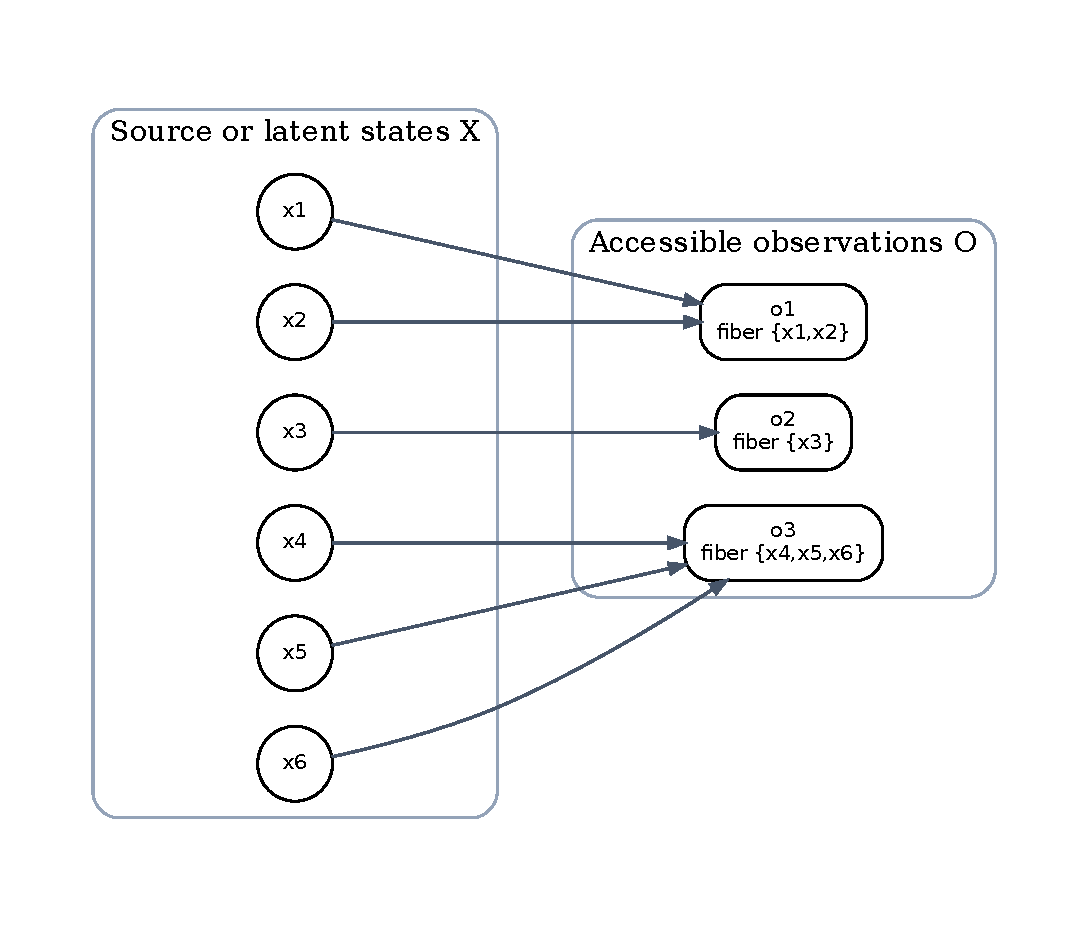
\includegraphics[width=0.82\textwidth]{figures/concept_observation_fibers.pdf}
\caption{Observation fibers. States in one fiber produce the same accessible value. Fiber membership is relative to the specified map. A refined interface may split a fiber that a coarse interface leaves merged.}
\label{fig:observationfibers}
\end{figure}

The accessible value contains no internal tag selecting its source member. A reconstruction claim must therefore use an injective interface, an independently justified restriction on the source class, or additional information supplied from outside the current observation value.

\section{Related work}
\label{sec:relatedwork}

Which properties of a system can an observer recover from a measurement? Observability, statistical inference, and theories of perception approach this question with different definitions of a measurement. Each theory specifies what the observer can record.

\subsection{Observability and identifiability}

In control theory, an output trajectory can carry information about a state that a single reading omits. Kalman studied state recovery in linear systems \parencite{Kalman1963}. Hermann and Krener studied observability in nonlinear systems \parencite{HermannKrener1977}. In structural identifiability, the unknown quantity may be a parameter or a model structure \parencite{BellmanAstrom1970,Rothenberg1971,WalterPronzato1997}. Two parameter choices can agree on every ideal observation. Noise and limited sampling can also make distinguishable parameters difficult to estimate \parencite{Calderon1980,Raue2009,Chis2011,Villaverde2016,Meshkat2009,Guillaume2019}.

A nontrivial observation fiber gives a specific form of nonuniqueness. Several states produce the same reading. Well-posedness also requires existence and stability of the solution \parencite{Hadamard1923,Tikhonov1963,Engl1996}. Regularization can select one state in a fiber. A claim that the measurement identifies that state requires an additional assumption or observation.

Latent-variable models likewise require conditions for uniqueness \parencite{Teicher1963,Kruskal1977,Allman2009,Anandkumar2014}. In unsupervised learning, distinct latent representations can agree on the observations \parencite{Locatello2019}. Auxiliary variables, multiple views, and restrictions on the model can restore identifiability in specified settings \parencite{Hyvarinen2019,Khemakhem2020,Gresele2020,XiBloemReddy2023}. Tenenbaum and colleagues describe how learners acquire structured abstractions from data \parencite{Tenenbaum2011}. In the deterministic model, adding an unread coordinate gives an explicit example of two latent representations with the same reachable observations.

\subsection{Equivalence under a family of tests}

The information available to an experiment determines which systems it can distinguish. Blackwell compares statistical experiments by their informativeness for decisions \parencite{Blackwell1951,Blackwell1953,Torgersen1991}. Moore experiments and bisimulation compare states by specified external behavior \parencite{Moore1956,Park1981,Milner1989,LarsenSkou1991,Rutten2000}. In causal analysis, interventions can separate graphs that have the same observational conditional independences \parencite{VermaPearl1990,Chickering1995,Andersson1997,Pearl2009,HauserBuhlmann2012}. An observation-only experiment in the deterministic model receives a single reachable output. Equality of reachable sets constrains those experiments. Comparing event probabilities or temporal records requires a model that assigns them.

\subsection{Appearance, perspective, and hidden order}

Philosophical accounts of perception distinguish an appearance from the conditions that produce it. Plato's cave illustrates how a display can reveal only part of its source \parencite{Plato1992}. Aristotle distinguishes several senses of cause \parencite{Aristotle1984}. Husserl asks how scientific objects acquire their meaning through intentional activity and the lifeworld \parencite{Husserl1970}. In an observation model, the distinction has a measurable consequence. Different source states can produce one accessible representation.

Leibniz asks what grounds a distinction between things and whether distinct entities can share all their properties \parencite{Leibniz1989,LeibnizClarke2000}. His account of perspective gives each monad a particular view of one world. Restricting the question to properties accessible through a map changes its answer. Two states in one fiber agree on every predicate that depends only on the reading. A predicate defined on the source can still distinguish them.

Whitehead describes reality through processes and relations \parencite{Whitehead1978}. Bohm's implicate order and his work with Hiley relate observable phenomena to a deeper physical process \parencite{Bohm1980,BohmHiley1993}. A hidden extension requires only a state coordinate omitted by the readout. A physical interpretation of that coordinate requires a model of how the coordinate affects measurable behavior.

\subsection{Formal limits and mechanical proof}

Diagonal arguments place limits on what particular formal systems can express. Cantor constructs an object outside a proposed enumeration \parencite{Cantor1891}. Russell identifies a contradiction in unrestricted set formation \parencite{Russell1908}. G\"odel establishes incompleteness under conditions on a formal theory \parencite{Godel1931}. Tarski gives conditions under which truth cannot be defined within the same language \parencite{Tarski1936}. Lawvere formulates a categorical fixed-point principle \parencite{Lawvere1969}. Hofstadter explores self-description in formal systems and minds \parencite{Hofstadter1979,Hofstadter2007}. Penrose proposes a disputed connection between G\"odelian limits and human cognition \parencite{Penrose1989,Penrose1994}. For a measurement, the obstruction to exact state recovery can be tested by asking whether two allowed states give the same reading.

Leibniz proposed a symbolic calculus for reasoning \parencite{Leibniz1989}. Modern proof assistants check whether a conclusion follows from encoded premises and inference rules. Lean and mathlib support this kind of verification \parencite{deMoura2015,Mathlib2020}. The Flyspeck project applied mechanical checking to a geometric proof \parencite{Hales2017}. A proof about a readout establishes a property of the specified map. Applying it to an instrument also requires evidence that the map describes the instrument's readings.

\subsection{Feedback and embedded observation}

An embedded observer can act on the system it observes. Wiener studied communication, control, and feedback \parencite{Wiener1948}. Ashby related the variety of disturbances to the responses available to a regulator \parencite{Ashby1956}. Second-order cybernetics includes the observer in the system under study \parencite{VonFoerster1981}. Autopoiesis and relational biology examine how a living system maintains its organization \parencite{MaturanaVarela1980,Rosen1991}. Von Neumann's work on measurement and self-reproducing automata links physical operations to descriptions of those operations \parencite{VonNeumann1955,VonNeumann1966}.

An external analyst can specify a readout without specifying its effect on the system. A model of an embedded observer must also describe how a reading changes later states or actions. Elshatlawy and colleagues propose operational equivalences and complexity measures for observers \parencite{Elshatlawy2025}. Abramsky and colleagues identify time, self-reference, and self-modification as open problems for models of living systems \parencite{Abramsky2025}.

\subsection{Information, scale, and physical computation}

Information theory quantifies distinctions that survive transmission and processing \parencite{Shannon1948a,Shannon1948b,KullbackLeibler1951,CoverThomas2006}. Theories of self-organization and emergence address how constraints and stable structures persist across scales \parencite{NicolisPrigogine1977,Kauffman1993,Deacon2011,Mitchell2009}. Hierarchical active inference constructs coarse states and paths across levels \parencite{Friston2025ScaleFree}. Applying the deterministic quotient at two scales requires an explicit map between them. A quantity on the finer states descends to the coarser states exactly when it is constant on each fiber.

A mathematical invariant and its physical interpretation have separate conditions. Hilbert's axioms admit geometric realizations that satisfy the same relations \parencite{Hilbert1902}. Newtonian mechanics and special relativity specify the changes of description under which their predictions agree \parencite{Newton1999,Einstein1905}. Physical predictions can then be tested against measurements \parencite{Feynman1965}. Wheeler considered the role of observation in physical description \parencite{Wheeler1983}. Constructor theory expresses physical laws in terms of possible and impossible transformations \parencite{Deutsch2013,DeutschMarletto2015}. Tegmark proposes information-processing properties for consciousness as a state of matter \parencite{Tegmark2015}. Wolfram describes bounded observers that combine computational histories into a single description \parencite{Wolfram2002,Wolfram2023ObserverTheory,RicklesEtAl2023}. Each proposal assigns its own physical or computational meaning to an observation.

A device's encoding and readout determine which abstract calculation its physical evolution implements. Shannon's differential analyzer uses continuous physical evolution for analog calculation \parencite{Shannon1941}. Horsman and colleagues make the relation between physical states and abstract computation explicit \parencite{Horsman2014,Horsman2015}. Quantum computation distinguishes preparation, controlled evolution, measurement, and classical output \parencite{DiVincenzo2000,AharonovCotlerQi2022}. Brain--computer interfaces use selected neural signals to generate device commands \parencite{Wolpaw2002,Willett2023}. Two devices can thus agree on the output of a computation while differing in substrate, noise, or accessible internal state.

\subsection{Consciousness, agency, and report}

A report is one observation of a subject under specified conditions. Chalmers distinguishes functional accounts from an explanation of subjective experience \parencite{Chalmers1995}. Theories of integration, global availability, attention, resonance, and predictive processing propose different relations among neural activity, report, and experience \parencite{Tononi2008,Koch2019,Graziano2013,Grossberg2021,Friston2010,Parr2022}. Jaynes proposed a historical account of self-modeling and source attribution \parencite{Jaynes1976}. Hoffman and Prakash distinguish perceptual interfaces from the objective structures that produce their outputs \parencite{HoffmanPrakash2014,PrentnerHoffman2024}. Theories of agency also distinguish levels of description. Sapolsky emphasizes the causal history of an action. List, Dennett, and Frankfurt describe forms of agency compatible with physical causation \parencite{Sapolsky2023,List2019,Dennett2003,Frankfurt1971}.

An experiment distinguishes theories when they predict different accessible outcomes \parencite{GomezMarinSeth2025,TononiEtAl2025}. The COGITATE collaboration preregistered divergent predictions of integrated information theory and global neuronal workspace theory. Its results challenged predictions of both \parencite{Cogitate2025}. Laukkonen, Friston, and Chandaria propose a recursively shared world model and precision control as conditions for consciousness \parencite{Laukkonen2025}. Whyte and colleagues formulate a minimal testable theory within active inference \parencite{Whyte2026}. Robinson and colleagues propose comparing active gaze shifts with passive replay of the same visual displacement \parencite{Robinson2025}. The assigned condition supplies a record separate from the participant's report that the target reappeared.

Artificial systems can expose different information through a verbal report, an internal state, and a monitoring channel. Chalmers examines possible routes to consciousness in language models \parencite{Chalmers2023LLM}. Butlin and colleagues propose indicators drawn from neuroscientific theories \parencite{ButlinEtAl2023}. Testing an indicator requires a channel that distinguishes the internal states on which the indicator takes different values.

\subsection{Neural manifolds and biological measurements}

Grid-cell studies recover population geometry from recordings and behavioral measurements \parencite{Gardner2022}. Related studies examine toroidal organization during one-dimensional behavior and the role of oscillatory dynamics in the recovered topology \parencite{Hermansen2024,DiSarra2025}. Spike sorting, behavioral sampling, and dimensionality reduction each restrict the available record. A published correction replaced duplicated panels in the synthetic torus calibration figure of the oscillation study \parencite{DiSarra2025Correction}. The robustness of a recovered neural manifold can be tested by varying the sampling and preprocessing and comparing the resulting topology.

Ultraweak photon emission supplies a different biological measurement. Research reports spontaneous emission from DNA under controlled conditions, differences between living and dead mice, and stress-related changes in plants \parencite{PietruszkaMarzec2024,Salari2025}. Detection methods and biological applications depend on the sources and intensities of the emissions \parencite{Mould2024}. The hypothesis that light carries information about living organization requires a specified property of that organization and a test of which emission readings distinguish its values.

\subsection{Observable state and empirical model class}

An observation map partitions states into fibers. A target can be recovered from a reading exactly when it is constant on the corresponding fiber. At the model level, equality of reachable sets groups models that admit the same observation labels. An unread coordinate can change the latent structure and prevent exact state recovery while preserving this reachable set. A second measurement improves recovery precisely when it separates the states that disagree on the target.

\section{Broader applications and research hypotheses}
\label{sec:limitations}

This appendix retains the broader research program. Its hypotheses are not consequences of the reconstruction theorem. The formal framework is exact, deterministic, static, and intentionally bounded. The limitations below define both the assumptions required for broader applications and the research program that follows.

\subsection{Set-based empirical equivalence and exact equality}

Empirical equivalence is equality of reachable observation sets. Real measurements include probabilities, frequencies, noise, finite precision, and time dependence. Two models can have the same support and different probability laws. A stochastic extension should assign measures or kernels to latent and observation spaces. Approximate equivalence should replace exact fibers by metric neighborhoods, couplings, or reconstruction-error bounds.

\subsection{Static interfaces and unrestricted hidden factors}

A dynamical trajectory can distinguish states that one instantaneous output cannot. Future formalization must include state evolution, inputs, intervention, and complete traces. The hidden-factor construction is also deliberately broad. Domain physics, causal structure, conservation laws, geometry, regularity, or minimality may exclude many extensions. The theorem states only that reachable-set equality does not exclude them by itself.

\subsection{Composite chains and local loss analysis}

The conceptual architecture contains apparatus, sampling, encoding, biological access, internal representation, report, and feedback. The current formal core composes these stages into one map. A richer theory should represent each stage and determine where a distinction is preserved, transformed, compressed, dispersed, or collapsed. Such a theory would permit local refinement of one stage and would show whether a later result contains new information or only a re-encoding of an earlier accessible state.

\subsection{The embedded self-interface}

The present analyst stands outside the declared map. Wiener, von Foerster, Maturana and Varela, Rosen, von Neumann, and recent computational observer programs supply distinct precedents for treating observation, self-production, and feedback as coupled rather than external operations \parencite{Wiener1948,VonFoerster1981,MaturanaVarela1980,Rosen1991,VonNeumann1966,Wolfram2023ObserverTheory,RicklesEtAl2023}. The next major formal problem is an embedded system \(S\) that contains a self-model and uses the output of a self-interface to update its own dynamics:
\[
S_t\xrightarrow{\pi_{\mathrm{self}}}O^{\mathrm{self}}_t
\xrightarrow{u}S_{t+1}.
\]
The question is not merely whether \(\pi_{\mathrm{self}}\) is injective. It is whether the system can justify the interface and update rule using only resources generated inside the same process. Coalgebra, domain theory, second-order cybernetics, and active inference are candidate tools \parencite{VonFoerster1981,Abramsky2025,Friston2025ScaleFree}. No general self-justification theorem is claimed here.

\subsection{Cross-domain candidate invariant}

The candidate invariant should be tested separately in logic, computation, cognition, language, biology, artificial intelligence, and physics:
\begin{quote}
\emph{No sufficiently expressive representational system can completely justify or perceive the boundary that generates its own representational capacity.}
\end{quote}
A successful program must define \emph{system}, \emph{representation}, \emph{boundary}, \emph{justify}, and \emph{complete} in each domain, then identify a common theorem or explain why the analogy fails. G\"odel, Tarski, Lawvere, cybernetics, generalized-observer proposals, and self-referential biology supply test cases rather than proof of universality \parencite{Godel1931,Tarski1936,Lawvere1969,Elshatlawy2025,Abramsky2025}.

\subsection{Paradox as a boundary signal}

\begin{hypothesis}[Boundary-signal hypothesis]
A recurrent paradox may sometimes mark a representational system encountering the limit of its own closure rather than an ordinary contradiction inside the model.
\end{hypothesis}
The hypothesis requires a classifier that distinguishes inconsistent assumptions, semantic ambiguity, formal undecidability, empirical underdetermination, and changed access conditions. It is weakened or rejected if all candidate cases are explained by ordinary error without residual structure. It gains support only if a formally defined boundary measure predicts where otherwise independent paradox-like failures occur.

\subsection{Observer-relative mathematics}

A further philosophical hypothesis is that mathematics arises through interaction between an observer and reality, while shared mathematics records structures that remain invariant across different representational routes. In its strongest informal form, ``what we call mathematics is what observers can preserve and agree upon.'' This is not implied by the formal theorem. Mathematical structuralism and category-theoretic invariance provide relevant comparison points \parencite{Shapiro1997,Leinster2014}. Hilbertian axiomatics separates a structure from one concrete realization, while Newtonian and Einsteinian physics illustrate how stable law or invariant relation can survive changes of coordinates and representation \parencite{Hilbert1902,Newton1999,Einstein1905}. Feynman's account of physical law supplies a further methodological reminder that mathematical form earns physical force only through contact with experiment \parencite{Feynman1965}. A future paper would need to distinguish conventional notation, structural equivalence, proof-theoretic invariance, and observer-dependent access to mathematical objects.

\subsection{Materialism, constraint, and unified-state formation}

\begin{hypothesis}[Constraint and unified-state hypothesis]
A physical account of consciousness is incomplete unless it explains how high-dimensional activity is constrained into a stable, integrated, reportable regime rather than merely listing the participating components.
\end{hypothesis}
This hypothesis is not the claim that matter cannot produce consciousness. It asks which dynamical constraints, integration mechanisms, or model-selection processes make a system behave as one temporally coherent state. Hard determinist arguments emphasize the causal closure of biological history, while compatibilist accounts locate agency at the level of reasons, alternatives, control, or second-order endorsement \parencite{Sapolsky2023,List2019,Dennett2003,Frankfurt1971}. These positions do not settle consciousness, but they sharpen the requirement that constraint, agency, and reportability be defined at the correct level. Current active-inference, global-workspace, and integrated-information programs offer distinct answers and are now being subjected to prospective comparison \parencite{SethBayne2022,Cogitate2025,Laukkonen2025,Whyte2026,Robinson2025}. The interface analysis adds an identifiability question: do the proposed measurements distinguish the relevant internal mechanisms, or do multiple mechanisms remain in one empirical class?

A disconfirming outcome would be a sufficiently complete component-level account that predicts unified reportability without requiring an additional system-level constraint variable. A supporting result would require a defined constraint measure that predicts transitions in reportability across sleep, anesthesia, perturbation, or pathology better than competing explanations.

\subsection{Scale-conditioned death and observability}

\begin{hypothesis}[Scale-transition hypothesis of death]
Death is not annihilation of informational structure but a transition in which that structure is redistributed across scales and degrees of freedom, making it no longer observable as a coherent system at the original scale.
\end{hypothesis}
This is a proposed research stance, not a theorem. It must distinguish at least four possibilities: physical persistence of matter and energy, persistence of specific correlations, persistence of organism-level organization, and persistence of subject-level identity. Conservation of energy does not by itself imply conservation of organismal organization or recoverable personal information.

A valid study would define the original-scale coherence criterion, measure selected correlations before and after organismal death, vary spatial and temporal resolution, and determine whether apparent loss at one scale becomes structured signal at another. Failure to detect a structure cannot establish annihilation; detection of a transformed signal cannot establish continuity of the original organism without a reconstruction criterion.

\subsection{Light as an informational standard hypothesis}

\begin{hypothesis}[Light and living organization]
``Light is the informational standard of the living; when it turns into something else it is the informational standard of the dead.''
\end{hypothesis}
The statement is retained exactly as a named hypothesis because it motivated a proposed measurement route. It is not used as a physical fact. To become testable, \emph{informational standard} must be defined as a measurable statistic or family of statistics, and \emph{turns into something else} must specify energy transfer, spectral change, temporal correlation, spatial dispersion, or coupling to another degree of freedom.

Ultraweak photon emission provides one concrete but limited observable. Living and dead mice show measurable differences in ultraweak emission, and emissions in DNA, cultured cells, and stressed plants can be measured under controlled conditions \parencite{PietruszkaMarzec2024,Salari2025,Mould2024}. These observations neither establish a universal living/dead standard nor show that photon emission encodes complete organismal information. A future study should test whether emission statistics predict defined organization or viability measures beyond temperature, oxidative state, metabolic activity, and tissue composition.

\subsection{Single-observer, intentional-forgetting, and external-source hypotheses}

The broader metaphysical hypothesis can be stated without converting it into a conclusion: one foundational observer generates a contained reality, relinquishes control or memory, and experiences apparently independent beings through the system. Intentional forgetting is proposed as a condition that permits uncertainty, love, suffering, discovery, and nontrivial choice. A related external-source hypothesis asks whether structure outside the accessible system could leave internal traces through boundary conditions, invariants, or failures of closure.

These hypotheses are neither proved nor refuted by the present theorem. Their rule of admissibility is strict:
\[
\boxed{\text{No external-source hypothesis earns support without a discriminating prediction.}}
\]
A changed subjective sense of access, revelation, or certainty is not by itself a discriminating prediction. A valid test must specify an outcome unlikely under the physical, plural-observer, information-only, and cognitive alternatives. If no such outcome can be stated, the hypothesis remains metaphysical and must not be used to explain the formal result.

\subsection{Containment, internal reality, and meaning}

The interpretive application is that containment does not imply falseness. Experiences and relations may be real within a containing process even when their ontology is dependent. Meaning, beauty, freedom, and truth may be internally stable outputs of a system without being established as absolute outside it. This claim is philosophical rather than empirical. Leibnizian perspectivism, Whiteheadian relation, and Peircean fallibilism provide three different historical comparisons for this claim \parencite{Leibniz1989,Whitehead1978,Peirce1877,Peirce1878}. Future work should formalize it as invariance under a declared family of transformations: which relations remain stable across observers, interfaces, encodings, or scales?

\subsection{Identity, factorial zero, layered tensors, and geometry}

A separate mathematical note is reserved for the recurring motif that the unit value \(1\) appears as \(0!\), the empty product, \(e^0\), \(\Gamma(1)\), \(\det I\), probability normalization, and identity action. The proposed conceptual sequence is
\[
\text{preserved unit}\longrightarrow
\text{metric structure}\longrightarrow
\text{connection}\longrightarrow
\text{curvature}.
\]
The intended intuition is that Christoffel symbols arise when an identity-like metric structure varies across coordinates, and curvature arises from derivatives and products of the connection. For a specified smooth metric, the Levi-Civita connection depends on the metric and its first derivatives; curvature depends on the connection and its derivatives. Coordinate-dependent metric components can produce nonzero connection coefficients even in flat space, so they do not alone establish curvature. This geometric calculation must be developed independently \parencite{Nakahara2003}. It is not a result of the present theorem, and \(0!=1\) does not by itself generate a connection or curvature tensor.

\subsection{Neural manifolds and reportability}

Published reconstructions of grid-cell population activity motivate an application of the multi-stage interface problem \parencite{Gardner2022,Hermansen2024,DiSarra2025}. The source state, electrode signal, spike-sorted representation, behavioral alignment, dimensional reconstruction, topological summary, biological access, and verbal report are not one object. Future work should define the maps between these levels and test which topological and dynamical conclusions survive justified changes in sampling, preprocessing, reconstruction, and behavioral context.


\subsection{Heterogeneous computational and engineered interfaces}

The same abstract result should not be assumed to have the same meaning in a digital computer, analog device, quantum processor, brain--computer interface, biological observer, multisensor suite, guidance system, or particle detector. Each system has a different physical state space, encoding, admissible operation, error model, and readout. Future formal work should therefore represent a family of interface implementations
\[
(S_i,\eta_i,U_i,\rho_i)
\]
and ask when two implementations realize the same abstract map, when they are refinements of one another, and when an output equivalence conceals different internal processes.

Safety-critical systems make the issue concrete. A multisensor suite combines partial, noisy, and sometimes conflicting measurements into an estimated state or decision; the fusion output remains conditional on coverage, calibration, timing, uncertainty, and the selected fusion architecture \parencite{HallLlinas1997,DurrantWhyteHenderson2008}. An inertial guidance system acts from estimated position, velocity, attitude, and uncertainty rather than direct access to an external ground truth \parencite{Kalman1963,TittertonWeston2004}. A particle-physics exclusion contour is conditional on detector acceptance, reconstruction, the tested model, and a statistical rule \parencite{Cowan2011,ParticleDataGroup2026}. These cases should be formalized as different interface classes rather than treated as intuitive analogies alone.

\subsection{Technical development program}

The next mathematical developments are:
\begin{enumerate}[label=(\roman*)]
\item stochastic observation channels and equality of induced measures;
\item approximate equivalence and quantitative reconstruction error;
\item dynamical observability with inputs and interventions;
\item composition of multiple interfaces and stage-specific fiber analysis;
\item information measures for quotient size, dispersion, and refinement cost;
\item criteria for minimal or canonical representatives;
\item embedded self-interfaces with feedback and model revision;
\item automated countermodel and discriminating-experiment construction;
\item formal comparison with Leibnizian indiscernibility and perspectival representation;
\item computational-irreducibility and bounded-observer criteria;
\item artificial-system interfaces and machine-consciousness indicator tests;
\item translation maps among digital, analog, quantum, neural, and human computational interfaces;
\item state-estimation systems whose actions depend on an internal model and quantified error;
\item multisensor suites that combine partial observations into a bounded state estimate or decision;
\item particle-physics acceptance, blind-region, and exclusion analyses as distinct kinds of boundary claim; and
\item domain-specific applications with independently justified maps.
\end{enumerate}

\subsection{Hypothesis and application register}

\begingroup
\small
\begin{longtable}{@{}>{\raggedright\arraybackslash}p{0.18\textwidth}>{\raggedright\arraybackslash}p{0.17\textwidth}>{\raggedright\arraybackslash}p{0.26\textwidth}>{\raggedright\arraybackslash}p{0.29\textwidth}@{}}
\caption{Status and next requirement for each broader application.}\label{tab:hypothesisregister}\\
\toprule
Program & Current status & Required next object & What would count as progress \\
\midrule
\endfirsthead
\toprule
Program & Current status & Required next object & What would count as progress \\
\midrule
\endhead
Embedded boundary invariant & Cross-domain conjecture & Domain-specific definitions and a common translation theorem & A theorem recurring across at least two nontrivially different domains, or a counterexample that narrows the claim \\
Paradox as boundary signal & Hypothesis & Classifier separating error, undecidability, and empirical underdetermination & Prospective prediction of boundary failures not explained by ordinary inconsistency \\
Observer-relative mathematics & Philosophical hypothesis & Invariance class across formal languages or observers & A precise theorem connecting translation-invariant structure to interface equivalence \\
Constraint and unified consciousness & Empirical and computational program & Defined constraint or integration variable and competing models & Preregistered predictions across state transitions that separate mechanisms \\
Scale-conditioned death & Empirical hypothesis & Coherence criterion across scales and time & Measured transformed structure with a justified continuity or reconstruction relation \\
Light as informational standard & Not yet operationalized & Spectral, temporal, spatial, or information statistic & Predictive value beyond metabolic, thermal, and oxidative confounds \\
Single foundational observer & Metaphysical hypothesis & Unique discriminating prediction & An outcome not shared by plural-observer, physical, information-only, or cognitive alternatives \\
External source or revelation & Metaphysical hypothesis & Publicly checkable boundary condition or invariant & Reproducible evidence with lower likelihood under internal alternatives \\
Identity-to-geometry motif & Separate mathematical note & Independent differential-geometric derivation & Correct theorem showing the precise relation, or a clear statement of the analogy's limits \\
Leibnizian perspective and indiscernibility & Historical-formal comparison & Translation between all properties and interface-accessible predicates & A theorem specifying when interface equivalence preserves or fails Leibnizian indiscernibility \\
Process and constraint dynamics & Dynamical application program & State evolution, constraints, and measurable order parameters & A model separating process, constraint, and observation effects with falsifiable predictions \\
Computational irreducibility and observer theory & Comparative formal program & Explicit coarse-graining and resource bounds & A theorem relating computational aggregation to interface refinement or a counterexample separating them \\
Artificial-system observer interfaces & Empirical and ethical application & Declared outputs, hidden states, self-monitoring channels, and indicator criteria & Tests that distinguish report equivalence from mechanism or consciousness claims \\
Neural manifold and reportability & Empirical application & Explicit maps from neural activity through measurement and reconstruction to report & Results stable across justified preprocessing, sampling, reconstruction, and behavioral changes \\
Heterogeneous physical computation & Formal and engineering application & Encoding, evolution, and readout maps for each implementation & A theorem stating when digital, analog, quantum, neural, or human interfaces realize the same abstract relation \\
Inertial navigation and guidance & State-estimation application & Dynamical model, sensor map, error state, and uncertainty relation & Correct predictions of when distinct physical trajectories remain indistinguishable to the estimator \\
Multisensor suite and data fusion & Safety-critical state-estimation application & Sensor-specific observation maps, timing, uncertainty, and a declared fusion rule & Correctly calibrated estimates whose blind regions, residuals, and unresolved state components are explicit \\
Particle-physics forbidden and excluded regions & Experimental application & Separate definitions for theoretical prohibition, detector inaccessibility, and statistical exclusion & Reproducible limits whose dependence on model, acceptance, and confidence rule is explicit \\
\bottomrule
\end{longtable}
\endgroup

The distinction among theorem, computation, interpretation, empirical application, and metaphysical hypothesis must remain explicit.

\section{Motivation and broader questions}
\label{app:motivation}

\subsection{Observation from within a system}

An embedded observer uses its body, senses, instruments, memory, language, and inference rules to form a description of the world. Can it also determine how those means of representation condition its experience? Its evidence for that question must come through the same means of observation.


Philosophy offers several formulations of this question. Plato distinguishes appearances from what produces them. Aristotle distinguishes kinds of cause \parencite{Plato1992,Aristotle1984}. Husserl examines how the structure of experience enters scientific descriptions \parencite{Husserl1970}. Leibniz relates perspective to sufficient reason and the identity of indiscernibles \parencite{Leibniz1989,LeibnizClarke2000}. Peirce connects the meaning of a concept to its conceivable practical consequences \parencite{Peirce1877,Peirce1878}. Whitehead emphasizes processes and relations \parencite{Whitehead1978}.

The conjecture about self-observation is
\begin{quote}
\emph{No sufficiently expressive representational system can completely justify or perceive the boundary that generates its own representational capacity.}
\end{quote}
The conjecture concerns an observer that must account for its own access. Formal self-reference has related limits in logic and semantics \parencite{Cantor1891,Russell1908,Godel1931,Tarski1936,Lawvere1969,Hofstadter1979,Hofstadter2007}. Kant distinguishes the conditions of experience from objects considered independently of those conditions \parencite{Kant1998}. Second-order cybernetics includes the observer in the system it describes \parencite{Ashby1956,VonFoerster1981,MaturanaVarela1980}. Work on generalized observers and self-referential living systems asks how to formalize that relation \parencite{Elshatlawy2025,Abramsky2025}. A general result for embedded physical observers remains open.

\subsection{Recovery through a specified interface}

A restricted version of the question has an exact answer. Given a source space and a fixed observation map, which differences between source states can an observation distinguish?

Let \(X\) be a source state space, let \(O\) be an accessible observation space, and let \(\pi:X\to O\) be the observation map. When
\[
\pi(x_1)=\pi(x_2)
\qquad\text{for}\qquad
x_1\neq x_2,
\]
the shared reading identifies a fiber containing both states. A function of that reading can return at most one of them as its answer.

The reconstruction theorem assumes a specified interface. A hidden extension shows that the same outputs can arise from different latent models. Whether a particular physical system must have a noninjective self-interface remains a separate question.

\subsection{Competing models and the stopping rule}

Several hypotheses can account for an observer who experiences a limit on its access.
\begin{enumerate}[label=(\alph*)]
\item one foundational observer that generates a contained reality and relinquishes access to its own control;
\item many genuinely independent observers within a shared physical world;
\item a physical universe that produces bounded biological observers;
\item an information-based reality without a singular foundational observer; and
\item a cognitive model through which an embedded mind organizes severe uncertainty and self-reference.
\end{enumerate}
If these models have the same possible reports, those reports alone cannot determine which model produced them.

A comparison requires a difference in predictions.
\begin{quote}
\emph{Treat the single-observer model, intentional forgetting, revelation, and every external-source model as metaphysical hypotheses unless they produce a testable prediction that distinguishes them from competing models, including through different outcome probabilities.}
\end{quote}
Peirce and Popper relate inquiry to practical consequences and the possibility of failure \parencite{Peirce1877,Popper1959}. Preregistered tests of consciousness theories specify outcomes that distinguish the competing predictions \parencite{Cogitate2025,Robinson2025}.



\FloatBarrier
\bibliographystyle{plainnat}
\bibliography{references}
\end{document}
